\documentclass[12pt]{article}

\title{Calculating fractal sets in $n \geq 1$ embedding dimensions without the use of truncation}
\author{
Shawn Halayka\footnote{Independent -- sjhalayka@gmail.com}
}


\date{\today\;\currenttime}

\usepackage{datetime}
\usepackage{listings}
\usepackage{cite}
\usepackage{xcolor}
\usepackage{graphicx}
\usepackage{setspace}
\usepackage{amsmath}
\usepackage{url}
\usepackage{amsfonts}
\usepackage{caption}
\usepackage{subcaption}

\usepackage[margin=1in]{geometry}

%\doublespace

\begin{document}




\maketitle

\begin{abstract}
The theme of this research is an examination of the traditional multiplication operator, in the case of fractal sets in $n \geq 1$ embedding dimensions.
After this examination, an alternative, new multiplication operator is introduced.
The traditional multiplication operator has a time complexity of $O(n^2)$, whereas the new multiplication operator has a time complexity of $O(n)$.
Taking amortized costs into account, it is found that the new multiplication operator is more time-efficient where $n \geq 32$, using an optimizing C++ compiler.
There is no problem, other than concerns about time complexity, with the traditional multiplication operator.
It was hypothesized that there would be differences between the two multiplication operators.
These differences, and some similarities, between the two multiplication operators are visualized in terms of fractal sets, via OpenGL.
The C++ and Python code is available upon request.
\end{abstract}




\section{Introduction}

The story of the Julia set begins with the discovery of the $2$D complex numbers \cite{cardano}, the $4$D quaternions \cite{hamilton}, and the $8$D octonions \cite{graves}, etc.
These number types allow us to extend the real numbers into more than one embedding dimension, providing data that are meant to be visualized.
For instance, in 1918, war veteran Gaston Julia published his trailblazing work on iterative equations (e.g. self-mappings).
The result is the Julia set \cite{julia, fatou}, which is a set of vertices along an input grid in $n$D space that satisfy one particular mathematical criterion. This criterion is that, for each $n$D input vertex $A$, the magnitude 
\begin{equation}
\ell =\sqrt{A_0 A_0 + A_1 A_1 + ... + A_{(n-1)} A_{(n-1)}} = \sqrt{\sum _{i=0}^{n-1} A_i^2}
\end{equation}
remains less than some chosen threshold value while undergoing iteration.
Note that $A_0$, $A_1$, etc. are real numbers.
In essence, the magnitude is the square root of the vertex's inner product in Euclidean (e.g., rectilinear) space.
In this paper, the maximum iterations is $8$, and the threshold value is $4$.

The traditional iterative equation is the non-linear polynomial
\begin{equation}
A^{\prime} = A^2 + D.
\end{equation}
where $D$ is some constant.

After a long pause in time, during which we waited for the computational capability, we come to the works of Norton and Holbrook \cite{norton, holbrook}, in the 1980s, which revolutionized the visualization of the Julia set -- up until then, the quaternion Julia set had been unexplored territory.
The work of Hart et al. \cite{hart} did a wonderful job of ray tracing the quaternion Julia set, setting the bar high for subsequent visualizations of fractals in general.

Inevitably, in the 1990s, the octonion Julia set was explored by Griffin and Joshi \cite{griffin}, and by Dixon et al. \cite{dixon}.

Afterwards, Cheng and Tan, along with Wang and Sun, generalized the quaternion Julia set \cite{cheng, wang} by allowing for a variable exponent in the iterative equation, and then Wang and Jin extended this work \cite{wang2} to include all embedding dimensions $n \geq 1$ via truncation.

The Julia set continues to mystify us to this day -- its complexity and beauty are without rival in all of the mathematics.
Up until now, those studying the Julia set have traditionally stuck close to the basic number types: real, complex, quaternion, octonion, etc.
This is because each of these number types have a well-defined multiplication operator.
There is no such traditional number type in, say, $5$D, unless you truncate and lose data like in \cite{wang2}.

In order to fully sidestep the missing $5$D number type, we will define a new multiplication operator.

Although we discuss the $5$D number type in this paper, we could have easily enough discussed any $n$D number type, where $n \geq 1$ is not necessarily equal to a power-of-two (e.g. not necessarily 1, 2, 4, 8, etc.) -- the same principles apply to all embedding dimensions $n \geq 1$. 

A deeper exploration of the Julia set is given in Katunin's book \cite{katunin}.
Although Katunin's book, in Chapter 2.3, cautions against using the $16$D sedenion, $32$D pathion, etc. multiplication operators, we find that Wang and Jin \cite{wang2} make use of both the sedenion and pathion multiplication operators just fine while calculating slices of $16$D and $17$D fractal sets.






\section{Traditional multiplication and truncation}

The traditional multiplication operator for octonions, where $C = AB$, is:
\begin{equation}
\begin{split}
C_0 = A_0 B_0 - A_1 B_1 - A_2 B_2 - A_3 B_3 - A_4 B_4 - A_5 B_5 - A_6 B_6 - A_7 B_7, \\
C_1 = A_0 B_1 + A_1 B_0 + A_2 B_3 - A_3 B_2 + A_4 B_5 - A_5 B_4 - A_6 B_7 + A_7 B_6, \\
C_2 = A_0 B_2 - A_1 B_3 + A_2 B_0 + A_3 B_1 + A_4 B_6 + A_5 B_7 - A_6 B_4 - A_7 B_5, \\
C_3 = A_0 B_3 + A_1 B_2 - A_2 B_1 + A_3 B_0 + A_4 B_7 - A_5 B_6 + A_6 B_5 - A_7 B_4, \\
C_4 = A_0 B_4 - A_1 B_5 - A_2 B_6 - A_3 B_7 + A_4 B_0 + A_5 B_1 + A_6 B_2 + A_7 B_3, \\
C_5 = A_0 B_5 + A_1 B_4 - A_2 B_7 + A_3 B_6 - A_4 B_1 + A_5 B_0 - A_6 B_3 + A_7 B_2, \\
C_6 = A_0 B_6 + A_1 B_7 + A_2 B_4 - A_3 B_5 - A_4 B_2 + A_5 B_3 + A_6 B_0 - A_7 B_1, \\
C_7 = A_0 B_7 - A_1 B_6 + A_2 B_5 + A_3 B_4 - A_4 B_3 - A_5 B_2 + A_6 B_1 + A_7 B_0.
\end{split}
\end{equation}
Note that $A_0$, $A_1$, etc. are real numbers.

For reference, we define commutativity as the satisfaction of the equality $AB = BA$, associativity as $(AB)D = A(BD)$, and distributivity as $A(B + D) = AB + AD$.

Note that the real multiplication is represented by the first term of the first line in Eq. 3.
Using the aforementioned definitions, the real multiplication is commutative, associative, and distributive.
Additionally, the complex multiplication is represented by the first two terms of the first two lines.
The complex multiplication is commutative, associative, and distributive.
Likewise, the quaternion multiplication is represented by the first four terms of the first four lines.
The quaternion multiplication is not commutative, but it is associative and distributive.
The octonion multiplication is not commutative, but it is associative and distributive.

For $5$D traditional multiplication, like in \cite{wang2}, the last three components of the two operands are set to $0$ before each multiplication operation occurs, and the last three components of the product are set to $0$ after each multiplication occurs -- in other words, they are all truncated, and data are lost.

For further details on traditional multiplication, please see the books \cite{sedenion} and \cite{quaternion}.







\section{Definition of a few useful functions in $n$D}

In this paper, we treat each $n$D vertex $A$ as consisting of a $1$D scalar $A_0$ and an $(n - 1)$D vector $(A_1, ..., A_{(n-1)})$.
The magnitude measures are:
\begin{equation}
\ell_s = \sqrt{A_0 A_0 + A_1 A_1 + ... + A_{(n-1)} A_{(n-1)}} = \sqrt{\sum _{i=0}^{n-1} A_i^2},
\end{equation}
\begin{equation}
\ell_v = \sqrt{A_1 A_1 + ... + A_{(n-1)} A_{(n-1)}} = \sqrt{\sum _{i=1}^{n-1} A_i^2}.
\end{equation}
The $C = \exp(A)$ function calculates the exponentiation of base $e$ (e.g. Euler's constant): 
\begin{equation}
\begin{split}
C_0 &= \exp(A_0) \cos(\ell_v), \\
C_1 &= \frac{A_1}{\ell_v} \exp(A_0) \sin(\ell_v), \\
...\\
C_{(n-1)} &= \frac{A_{(n-1)}}{\ell_v} \exp(A_0) \sin(\ell_v).
\end{split}
\end{equation}
Note that $A_0$, $A_1$, etc. are real numbers, and that these individual instances of $\exp()$, $\cos()$, $\sin()$ etc. are the familiar $1$D real-valued functions.
The $C = \log(A)$ function calculates the inverse of the exponentiation of base $e$:
\begin{equation}
\begin{split}
C_0 &= \log(\ell_s), \\
C_1 &= \frac{A_1}{\ell_v} \arccos\left( \frac{A_0}{\ell_s} \right), \\
...\\
C_{(n-1)} &= \frac{A_{(n-1)}}{\ell_v} \arccos\left( \frac{A_0}{\ell_s} \right).
\end{split}
\end{equation}
The $C = \sin(A)$ function is:
\begin{equation}
\begin{split}
C_0 &= \sin(A_0) \cosh(\ell_v), \\
C_1 &= \frac{A_1}{\ell_v} \cos(A_0) \sinh(\ell_v), \\
... \\
C_{(n-1)} &= \frac{A_{(n-1)}}{\ell_v} \cos(A_0) \sinh(\ell_v).
\end{split}
\end{equation}

For instance, where $n = 5$, the $C = \exp(A)$ function is:
\begin{equation}
\begin{split}
C_0 &= \exp(A_0) \cos(\ell_v), \\
C_1 &= \frac{A_1}{\ell_v} \exp(A_0) \sin(\ell_v), \\
C_2 &= \frac{A_2}{\ell_v} \exp(A_0) \sin(\ell_v), \\
C_3 &= \frac{A_3}{\ell_v} \exp(A_0) \sin(\ell_v), \\
C_4 &= \frac{A_4}{\ell_v} \exp(A_0) \sin(\ell_v),
\end{split}
\end{equation}
the $C = \log(A)$ function is:
\begin{equation}
\begin{split}
C_0 &= \log(\ell_s), \\
C_1 &= \frac{A_1}{\ell_v} \arccos\left( \frac{A_0}{\ell_s} \right), \\
C_2 &= \frac{A_2}{\ell_v} \arccos\left( \frac{A_0}{\ell_s} \right), \\
C_3 &= \frac{A_3}{\ell_v} \arccos\left( \frac{A_0}{\ell_s} \right), \\
C_4 &= \frac{A_4}{\ell_v} \arccos\left( \frac{A_0}{\ell_s} \right),
\end{split}
\end{equation}
and the $C = \sin(A)$ function is:
\begin{equation}
\begin{split}
C_0 &= \sin(A_0) \cosh(\ell_v), \\
C_1 &= \frac{A_1}{\ell_v} \cos(A_0) \sinh(\ell_v), \\
C_2 &= \frac{A_2}{\ell_v} \cos(A_0) \sinh(\ell_v), \\
C_3 &= \frac{A_3}{\ell_v} \cos(A_0) \sinh(\ell_v), \\
C_4 &= \frac{A_4}{\ell_v} \cos(A_0) \sinh(\ell_v).
\end{split}
\end{equation}

It should be noted that all we have done here is extend the $2$D complex functions (a part of the C++ language standard) into $5$D by including three extra imaginary components.








\section{Definition of a new multiplication operator in $n$D}

For both real and complex number types, where $A$ is not necessarily the same as $B$, it is known that 
\begin{equation}
C = A B = B A = \exp(\log(A) + \log(B)).
\end{equation}
We nominate this identity -- specifically $C = \exp(\log(A) + \log(B))$ -- as a new general-purpose commutative, associative, and distributive multiplication operator -- the multiplication operator without actual multiplication, for any embedding dimension $n \geq 1$.
For instance, all we need are the $5$D $\exp()$ and $\log()$ functions, which we defined in the previous section, and the addition operator, which in $5$D where $C = A + B$ is:
\begin{equation}
\begin{split}
C_0 &= A_0 + B_0, \\
C_1 &= A_1 + B_1, \\
C_2 &= A_2 + B_2, \\
C_3 &= A_3 + B_3, \\
C_4 &= A_4 + B_4.
\end{split}
\end{equation}








\section{Differences and similarities in terms of the products of the multiplication operators}

With regard to the new multiplication operator $C = \exp(\log(A) + \log(B))$ and the traditional multiplication operator $C = AB$: where $A = B$, the products of both operators are entirely similar for any $n \geq 1$.
It is where $A \neq B$ that the products are not necessarily entirely similar: sometimes the products are indeed entirely similar component-wise, sometimes only the magnitudes are similar, and sometimes they are not similar at all -- it all depends on $n$ and the individual components of $A$ and $B$.

Note that the traditional multiplication operator is generally not commutative, whereas the new multiplication operator is commutative.
Sets like 
\begin{equation}
A^{\prime} = \sin(A) + D \sin(A)
\end{equation}
are intriguing using both operators, and some resemblance can be seen -- see Figs. 1 and 2 for renderings of some $3$D slices of some $4$D fractal sets, which are generated by setting $A_3 = 0$ before the iteration function is called.

Note that both the new multiplication operator and the traditional multiplication operator produce the same result for
\begin{equation}
A^{\prime} = A^\beta + D, 
\end{equation}
where $\beta$ is an integer.
This is because $A^\beta$ and $A$ commute, in terms of the traditional multiplication operator (e.g. a special case due to the power associativity of traditional multiplication, where for instance $A(AA) = (AA)A$).
See Fig. 3 for a rendering of a $3$D slice of a $4$D fractal set, which is generated by setting $A_3 = 0$ before the iteration function is called.
Also see Figs. 4 and 5 for renderings of some $3$D slices of some $5$D fractal sets, which are generated by setting $A_3 = 0$ and $A_4 = 0$ before the iteration function is called.

These figures were rendered with OpenGL 4, using Phong shading and a shadow map.
For the full details on this rendering technique, please see Wolff's book \cite{wolff}.
The rendered triangle meshes were generated using Paul Bourke's marching cubes C++ implementation \cite{mc}, with a custom vertex interpolation function that helps to noticeably minimize aliasing.

Please see Figs. 6 - 9 for some graphs that compare the new multiplication product to the traditional multiplication product, for $A^{\prime} = A^2 + D$ and $A^{\prime} = \sin(A) + D \sin(A)$.





\section{Conclusion}

Here we have highlighted the existence of the Julia set in all $n \geq 1$ embedding dimensions, and not just a few dimensions like in the vast majority of previous works.
This is accomplished by introducing a new multiplication operator in all $n \geq 1$ embedding dimensions.
This technique is important because of its applicability and novelty.
For instance, we may use the new multiplication operator in general, for future work on topics other than the Julia set.

One nice thing about the new multiplication operator is that is doesn't rely on the traditional multiplication operator.
For instance, if we wished to try out, say, $9$D fractals, we wouldn't need to know the sedenion's non-commutative, non-associative, distributive traditional multiplication operator.

One other nice thing about the new multiplication operator is that it has a time complexity of $O(n)$ -- there is some small, constant number of multiplication operations for each of the $n$ components.
This is in comparison to the traditional multiplication operator (e.g. the one used in Eq. 9 in \cite{wang2}), which has a time complexity of $O(n^2)$ -- there are $n$ multiplication operations for each of the $n$ components.
The following table shows the amount of time, in seconds, that it takes to perform $10,000,000$ multiplication operations:
\begin{center}
\begin{tabular}{| l | r | r |}
  \hline
  Type & $O(n^2)$ time & $O(n)$ time \\
\hline
\hline
  Octonion $n = 8$ &1.8   &  4.3 \\
  Sedenion $n = 16$ & 2.9  & 4.9   \\
  Pathion $n = 32$ & 40.1  & 5.9   \\
  \hline  
\end{tabular}
\end{center}
Results may vary, but in general, for large $n$ (e.g. $n \geq 32$), the $O(n)$ method -- the new multiplication operator -- is the clear winner in terms of speed.
Here we used Microsoft Visual C++ (e.g. cl version 19.29.30133).

Thus, we have reason to investigate the new multiplication operator introduced in this paper, for it is truly $5$D -- no truncation is ever performed; no data are ever lost -- and it is inherently fast.


\section{Acknowledgments}

Thank you to Ricardo Fariello for introducing me to the quaternion pow() function.
Thank you to Paul Bourke for testing the math, and for coming up with preliminary figures.


\appendix





\section{Appendix: Fast exponentiation of variable base with the pow() function}

There is a pow() function of time complexity $O(n)$ that can replace many sequential multiplications where the exponent $\beta$ is an integer (e.g. in the case of $A$ multiplied by itself, again and again).
This makes for set calculation that is even faster than the new multiplication operator, especially for large $\beta$.

The magnitude measures are:
\begin{equation}
\ell_s = \sqrt{A_0 A_0 + A_1 A_1 + ... + A_{(n-1)} A_{(n-1)}} = \sqrt{\sum _{i=0}^{n-1} A_i^2},
\end{equation}
\begin{equation}
\ell_v = \sqrt{A_1 A_1 + ... + A_{(n-1)} A_{(n-1)}} = \sqrt{\sum _{i=1}^{n-1} A_i^2}.
\end{equation}
Where $\theta$ represents an angle in radians:
\begin{equation}
\theta = \beta \arccos \left(\frac{A_0}{\ell_s} \right),
\end{equation}	
the $C = {\textrm{pow}}(A, \beta)$ function in $n$D is:
\begin{equation}
\begin{split}
C_0 &= \ell_s^{\beta} \cos(\theta), \\
C_1 &= \frac{A_1}{\ell_v}\;\ell_s^{\beta} \sin(\theta), \\
... \\
C_{(n-1)} &= \frac{A_{(n-1)}}{\ell_v}\;\ell_s^{\beta} \sin(\theta).
\end{split}
\end{equation}
For instance, where $n = 5$, the $C = {\textrm{pow}}(A, \beta)$ function is:
\begin{equation}
\begin{split}
C_0 &= \ell_s^{\beta} \cos(\theta), \\
C_1 &= \frac{A_1}{\ell_v}\;\ell_s^{\beta} \sin(\theta), \\
C_2 &= \frac{A_2}{\ell_v}\;\ell_s^{\beta} \sin(\theta), \\
C_3 &= \frac{A_3}{\ell_v}\;\ell_s^{\beta} \sin(\theta), \\
C_4 &= \frac{A_4}{\ell_v}\;\ell_s^{\beta} \sin(\theta).
\end{split}
\end{equation}

See Fig. 10 for a $3$D slice of the $5$D Julia set, generated by using this pow() function.
Here we have set $A_3 = 0$ and $A_4 = 0$ before the iteration function is called.

Also, see Figs. 11 - 14 for $2$D slices of the $16$D Julia set.
Here we have set $A_2$ through $A_{15}$ to equal $0$ before the iteration function is called.

The following table shows the amount of time, in seconds, that it takes to perform $10,000,000$ multiplication operations versus $10,000,000$ pow() operations, where $\beta = 2$:
\begin{center}
\begin{tabular}{| l | r | r |}
  \hline
  Type & New multiplication time & pow() time \\
\hline
\hline
  Octonion $n = 8$ &4.3   &  2.2 \\
  Sedenion $n = 16$ & 4.9  & 2.3   \\
  Pathion $n = 32$ & 5.9  & 2.8   \\
  \hline  
\end{tabular}
\end{center}
The pow() function is twice as fast as the new multiplication operator, where $\beta = 2$.
As $\beta$ increases, the new multiplication operator becomes even slower by comparison.
For instance, where $\beta = 25$ for pathions, the pow() function is roughly $36$ times faster than the new multiplication operator.

This technique is important because of its applicability.
For instance, the technique is applicable to all linear and non-linear polynomials of the form 
\begin{equation}
A^{\prime} = X A^\beta + Y A^\gamma + ... + Z A + W.
\end{equation}
Only the pow() function (see Eq. 19), the new multiplication operator (see Eq. 12), and the addition operator (see Eq. 13) are required.

Note that $\beta$ need not be an integer in general, nor even a real.
For instance, we leave the exploration of $5$D exponents for future work, where:
\begin{equation}
A^\beta = \exp[\exp[ \log(\log(A)) + \log(\beta)]].
\end{equation}



\section{Appendix: Embedding versus fractal dimension}

Note that the embedding dimension $n$ is not the same thing as the fractal (e.g. box-counting) dimension of the set or its surface.

The box-counting dimension is calculated easily enough for $3$D slices of the $4$D and $5$D Julia sets.
One may run the magnitude data through the first half of the marching cubes algorithm, noting whether each marched cube (e.g. box) is along the surface or inside the set.
The marching cubes isovalue is equal to the threshold value.
If all 8 vertices of the marched cube correspond to a value less than the threshold, then the box is inside the set.
If only some of the vertices correspond to a value less than the threshold, then the box is along the surface.
Finally, if none of the vertices correspond to a value less than the threshold, then the box is outside the set.
Count the boxes accordingly, and use the marched cube side length $\ell_{\textrm{box}}$ to gather the box-counting dimension:
\begin{equation}
n_{\textrm{box}} = \lim_{\ell_{\textrm{box}} \to 0} \frac{ \log({\textrm{count}}(\ell_{\textrm{box}}))  }{\log\left(\frac{1}{\ell_{\textrm{box}}}\right)}.
\end{equation}
The basic idea is that the measure $n_{\textrm{box}}$ will become more and more accurate as $\ell_{\textrm{box}}$ goes to zero.
Note that the count is a function of the box size -- the smaller the boxes, the larger the count.

The triangles (e.g. simplices) need not be generated in the second half of the marching cubes algorithm, because all of the data that we need are already encoded in the marched cubes themselves.
This lack of simplices makes it very straightforward to extend the first half of the marching cubes algorithm to any embedding dimension $n \geq 1$ (e.g. marching hypercubes, where $n = 4$, but without the need for tetrahedra, or $n = 5$ but without pentachora, etc.), if one is not looking for mere slices.

Note that the fractal dimension $n_{\textrm{box}}$ need not be an integer like the embedding dimension $n$ is.


\section{Appendix: Artificial Intelligence}

The emulation of traditional multiplication can be performed by an artificial intelligence, namely an artificial neural network via the Python PyTorch package that performs non-linear regression.
Python acceleration can be enabled by using the Numba package, giving speeds similar to native C++.
In this paper we used Python 3.9.11, numpy 1.21.5, and numba 0.55.1.
Note that the artificial intelligence method is about an order or two of magnitude slower than the traditional multiplication, which is to be expected.
Output meshes are visualized in Fig. 15, showing promise for the artificial intelligence method.
The meshes were generated using the Python Scikit-image package's Lewiner marching cubes implementation.
We leave the exploration of hardware implementations of artificial neural networks for future work.




\pagebreak





\begin{thebibliography}{9}


\bibitem{cardano} Cardano. Ars magna. 1545
\bibitem{hamilton} Hamilton. On quaternions; or on a new system of imaginaries in algebra. 1843
\bibitem{graves} Graves. The mathematical papers of Sir William Rowan Hamilton. 1843
\bibitem{julia} Julia. M\'emoire sur l'it\'eration des fonctions rationnelles. 1918
\bibitem{fatou} Fatou. Sur les \'equations fonctionnelles. 1919

\bibitem{norton} Norton. Generation and display of geometric fractals in 3-D. Computer Graphics, 16(3):61–67, 1982
\bibitem{holbrook} Holbrook. Quaternionic asteroids and starfields, Applied Mathematical Notes, 8 (2), pp. 1-34, 1983
\bibitem{hart} Hart et al. Ray tracing deterministic 3-D fractals. Computer Graphics, 23(3):289–296, 1989

\bibitem{griffin} Griffin and Joshi. Octonionic Julia sets. Chaos Solitons and Fractals, 2(1):11–24, 1992
\bibitem{dixon} Dixon et al. Generation and graphical analysis of Mandelbrot and Julia sets in more than four dimensions. Computers \& Graphics, 20(3):451–456, 1996

\bibitem{cheng} Cheng and Tan. Generalization of 3D Mandelbrot and Julia sets. J Zhejiang Univ Sci A 2007 8(1):134-141s, 2006
\bibitem{wang} Wang and Sun. The general quaternionic M–J sets on the mapping $z \leftarrow z^a + c\;(a \in \mathbb{N})$. Computers \& Mathematics with Applications, 53(11) 1718–1732, 2007
\bibitem{wang2} Wang and Jin. Hyperdimensional generalized M–J sets in hypercomplex number space. Nonlinear Dynamics, 73(1):843–852, 2013

\bibitem{katunin} Katunin. A concise introduction to hypercomplex fractals. ISBN: 978-0367657642, 2017

\bibitem{sedenion} Imaeda and Imaeda, Sedenions: algebra and analysis, Applied mathematics and computation, vol. 115, pp. 77–88, 2000.

\bibitem{quaternion} Morais, Georgiev, Spr{\"o}{\ss}ig. Real Quaternionic Calculus Handbook. Basel: Birkh{\"a}user; 2014.

\bibitem{wolff} Wolff. OpenGL 4 Shading Language Cookbook - 3E. ISBN: 9781789342253, 2018

\bibitem{mc} Lorensen and Cline. Marching cubes: A high resolution 3D surface construction algorithm. ACM SIGGRAPH Computer Graphics. 21 (4): 163–169, 1987






\end{thebibliography}





\pagebreak






\begin{figure} 
\centering
  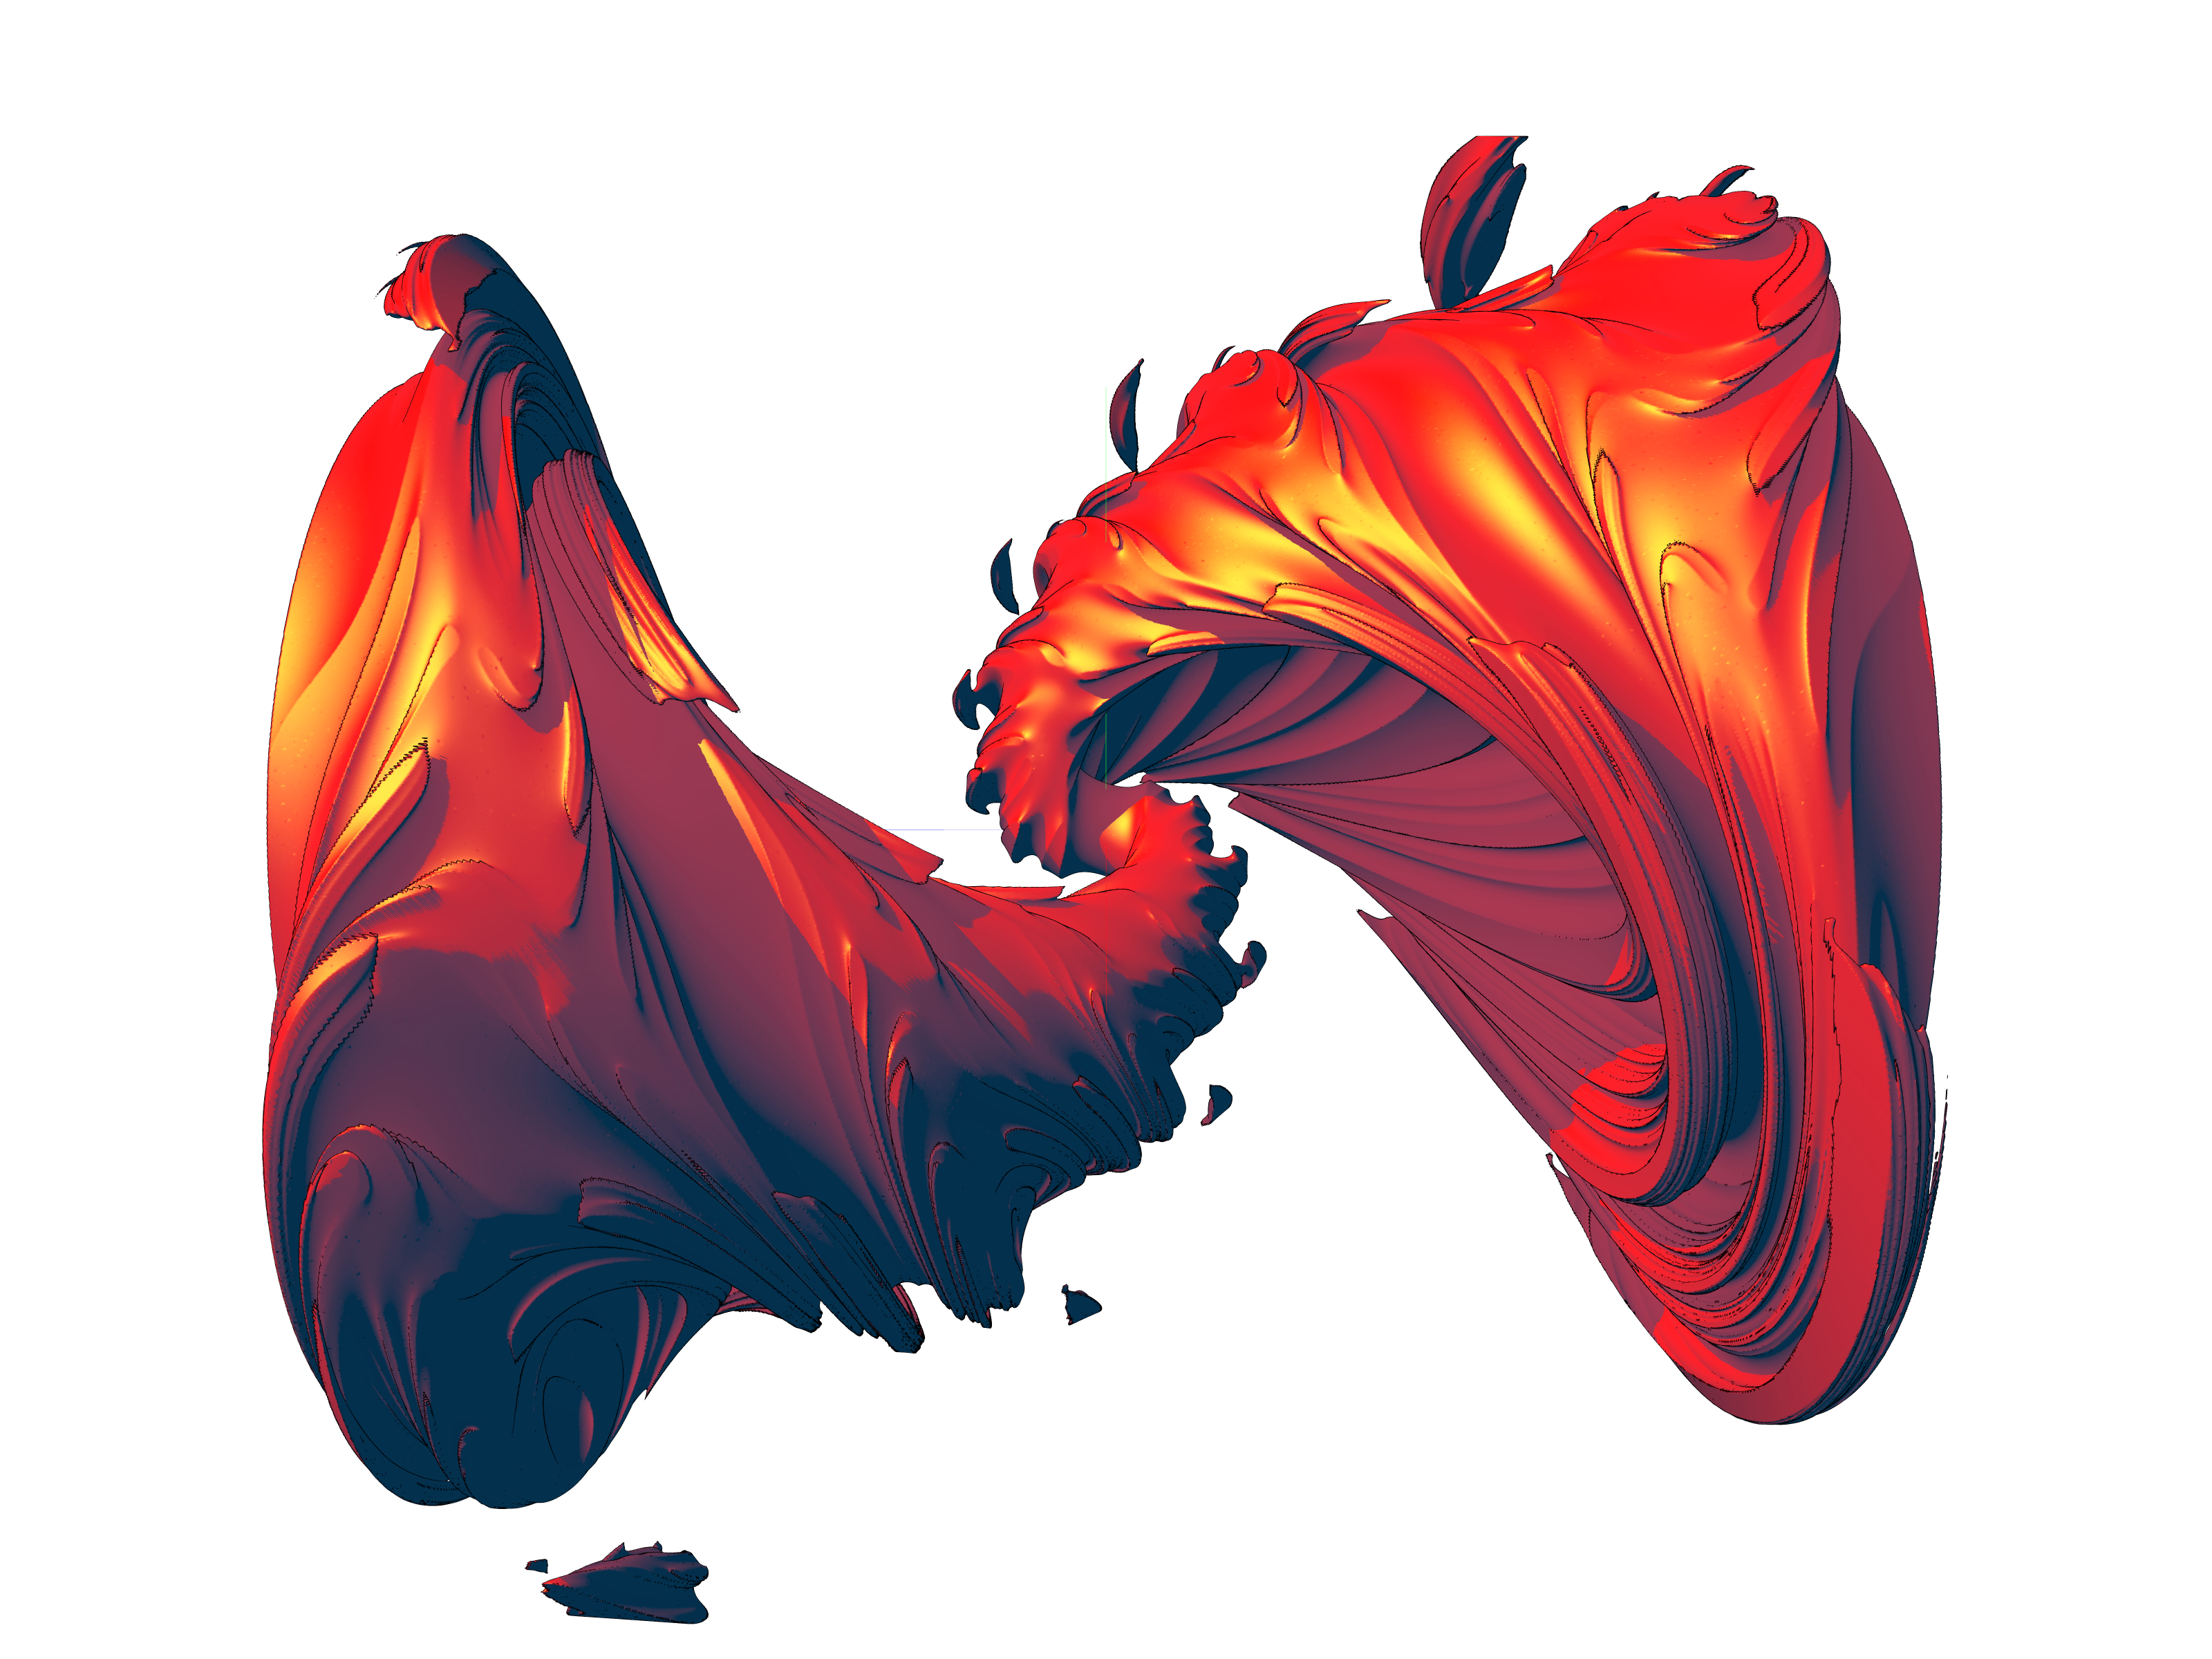
\includegraphics[width = 6 in]{quat_trad_mul.png}
  \caption{A rendering of a $3$D slice of a $4$D (e.g. quaternion) fractal set.
The iterative equation is $A^{\prime} = \sin(A) + D \sin(A)$, where $D = (0.3, 0.5, 0.4, 0.2)$.
The set is calculated using the traditional multiplication operator.
}
\end{figure}

\begin{figure} 
\centering
  \includegraphics[width = 6 in]{quat_new_mul.png}
  \caption{A rendering of a $3$D slice of a $4$D fractal set.
The iterative equation is $A^{\prime} = \sin(A) + D \sin(A)$, where $D = (0.3, 0.5, 0.4, 0.2)$.
The set is calculated using the new multiplication operator.
}
\end{figure}

\begin{figure} 
\centering
  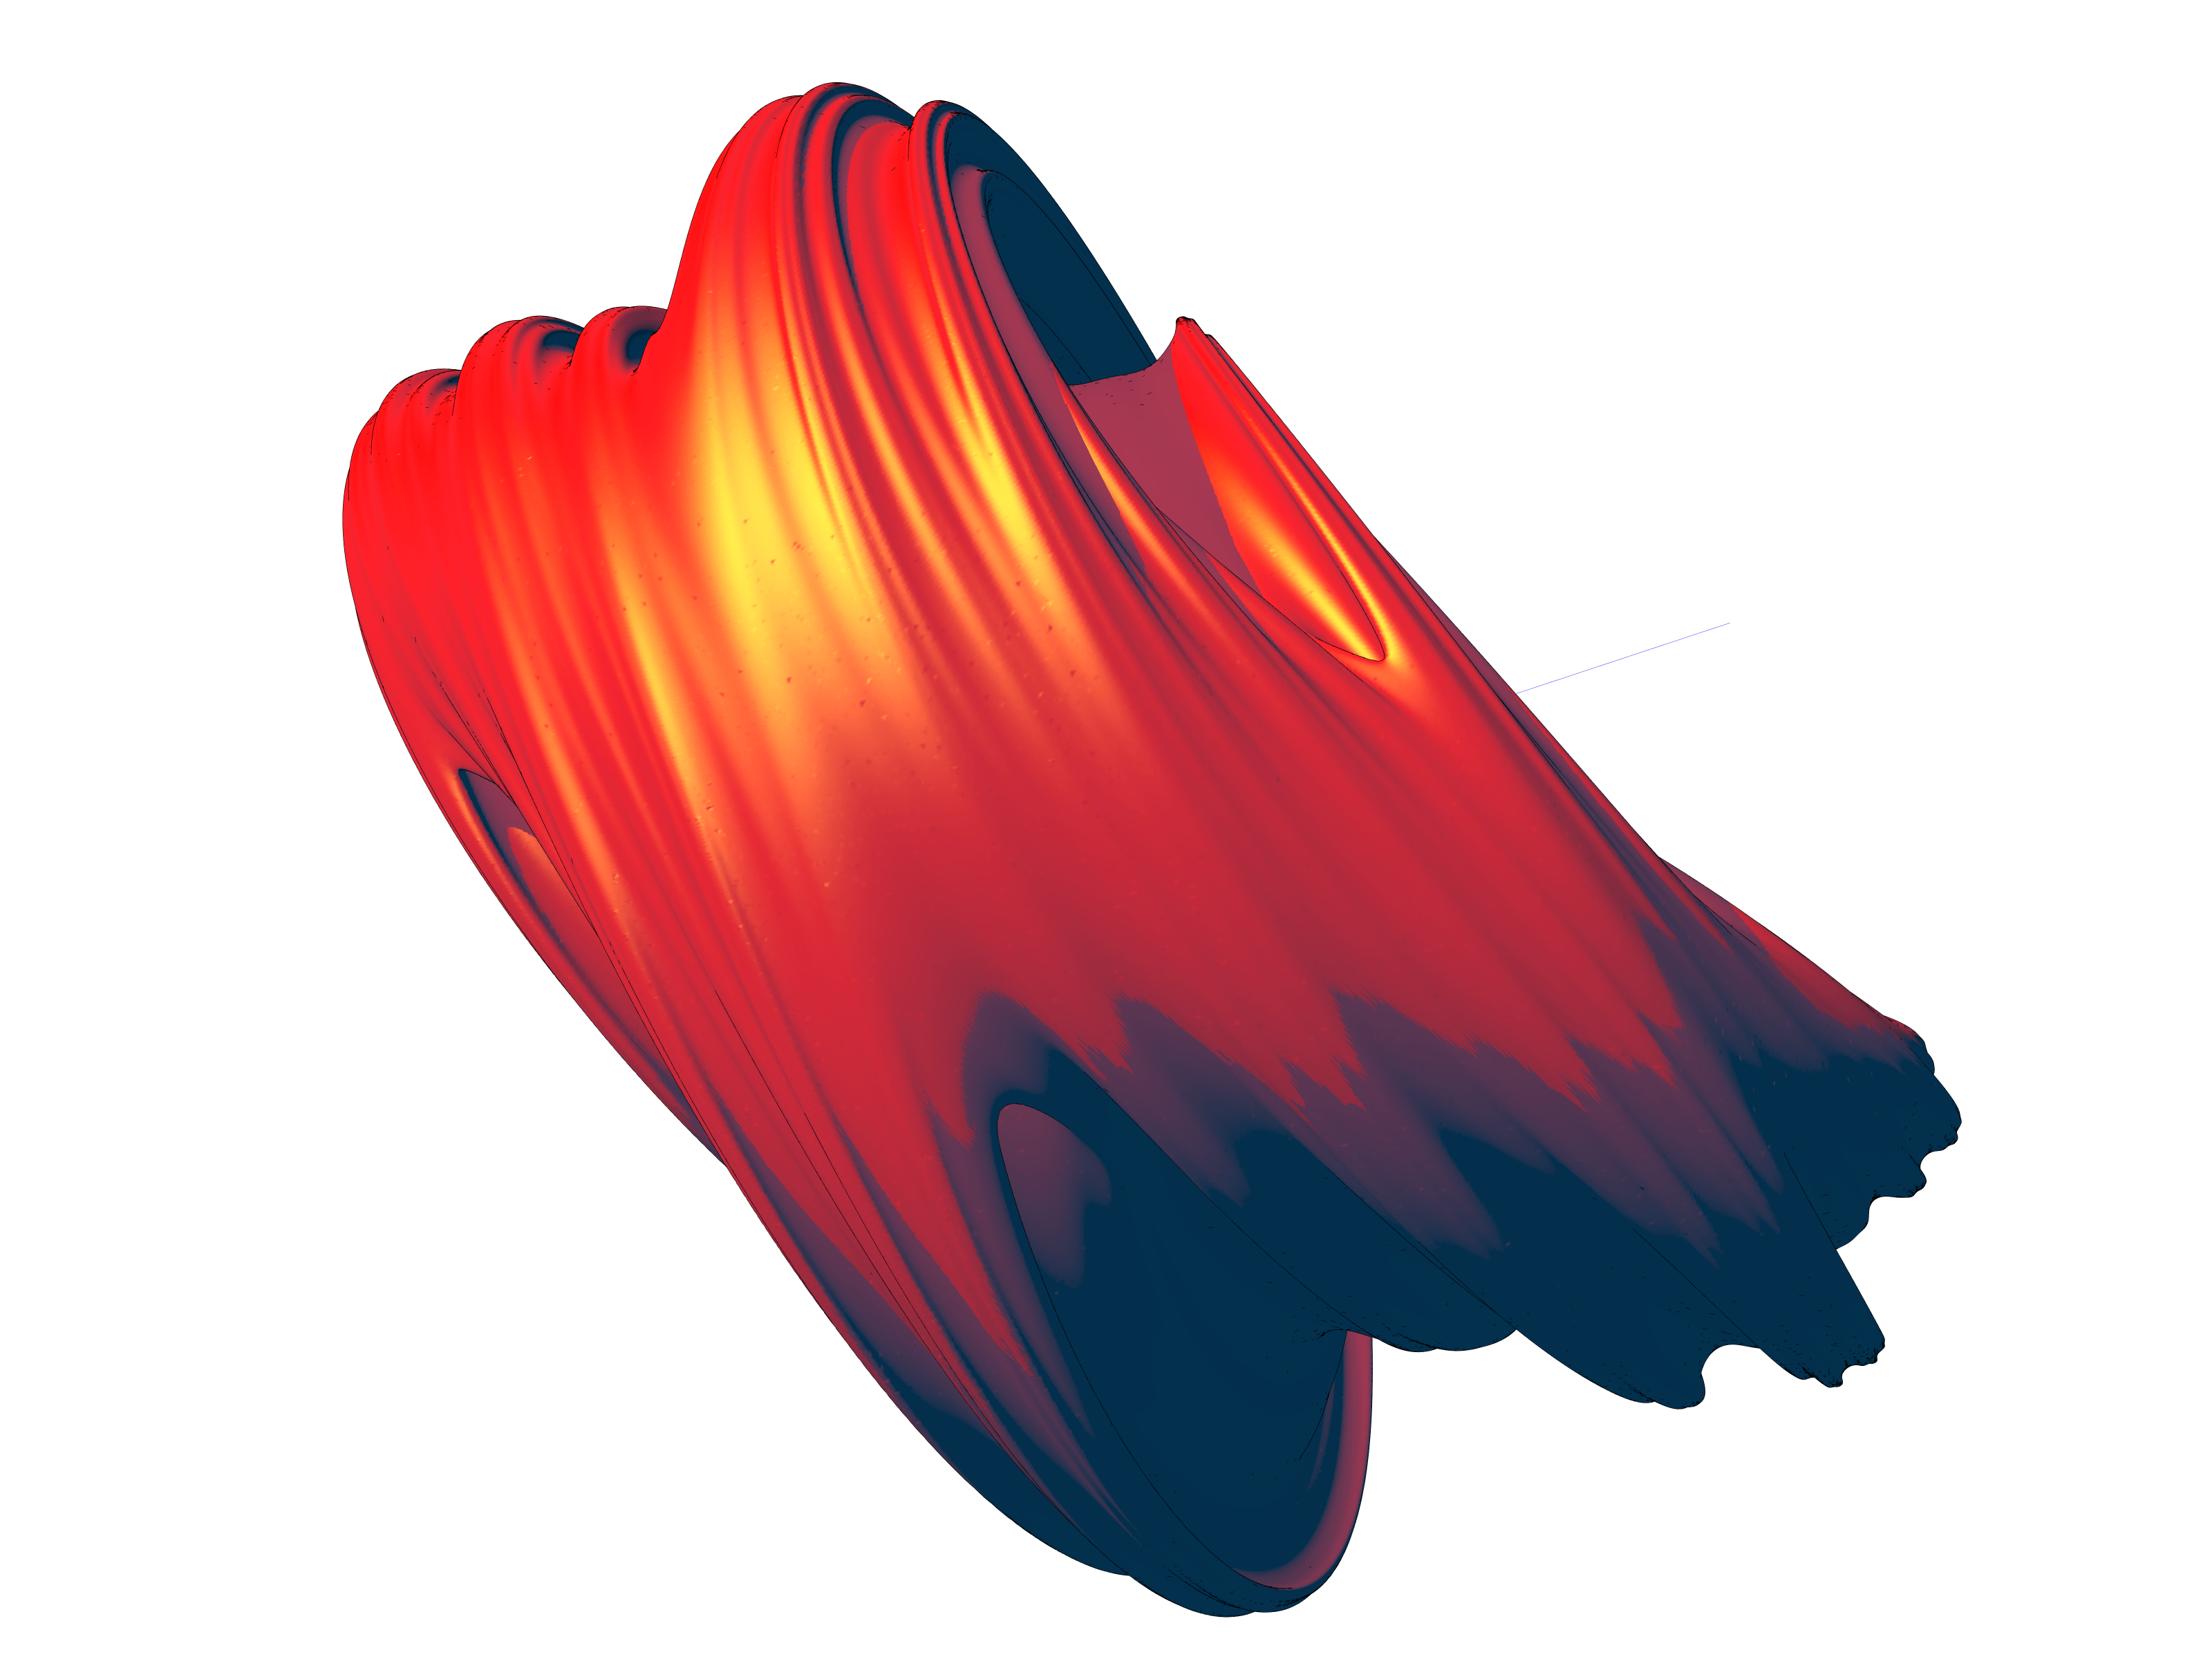
\includegraphics[width = 6 in]{quat_z2_c.png}
  \caption{A rendering of a $3$D slice of the $4$D Julia set.
The iterative equation is $A^{\prime} = A^2 + D$, where $D = (0.3, 0.5, 0.4, 0.2)$.
The set is calculated using the new multiplication operator, although the traditional multiplication operator generates the same set as well.
}
\end{figure}


\begin{figure} 
\centering
  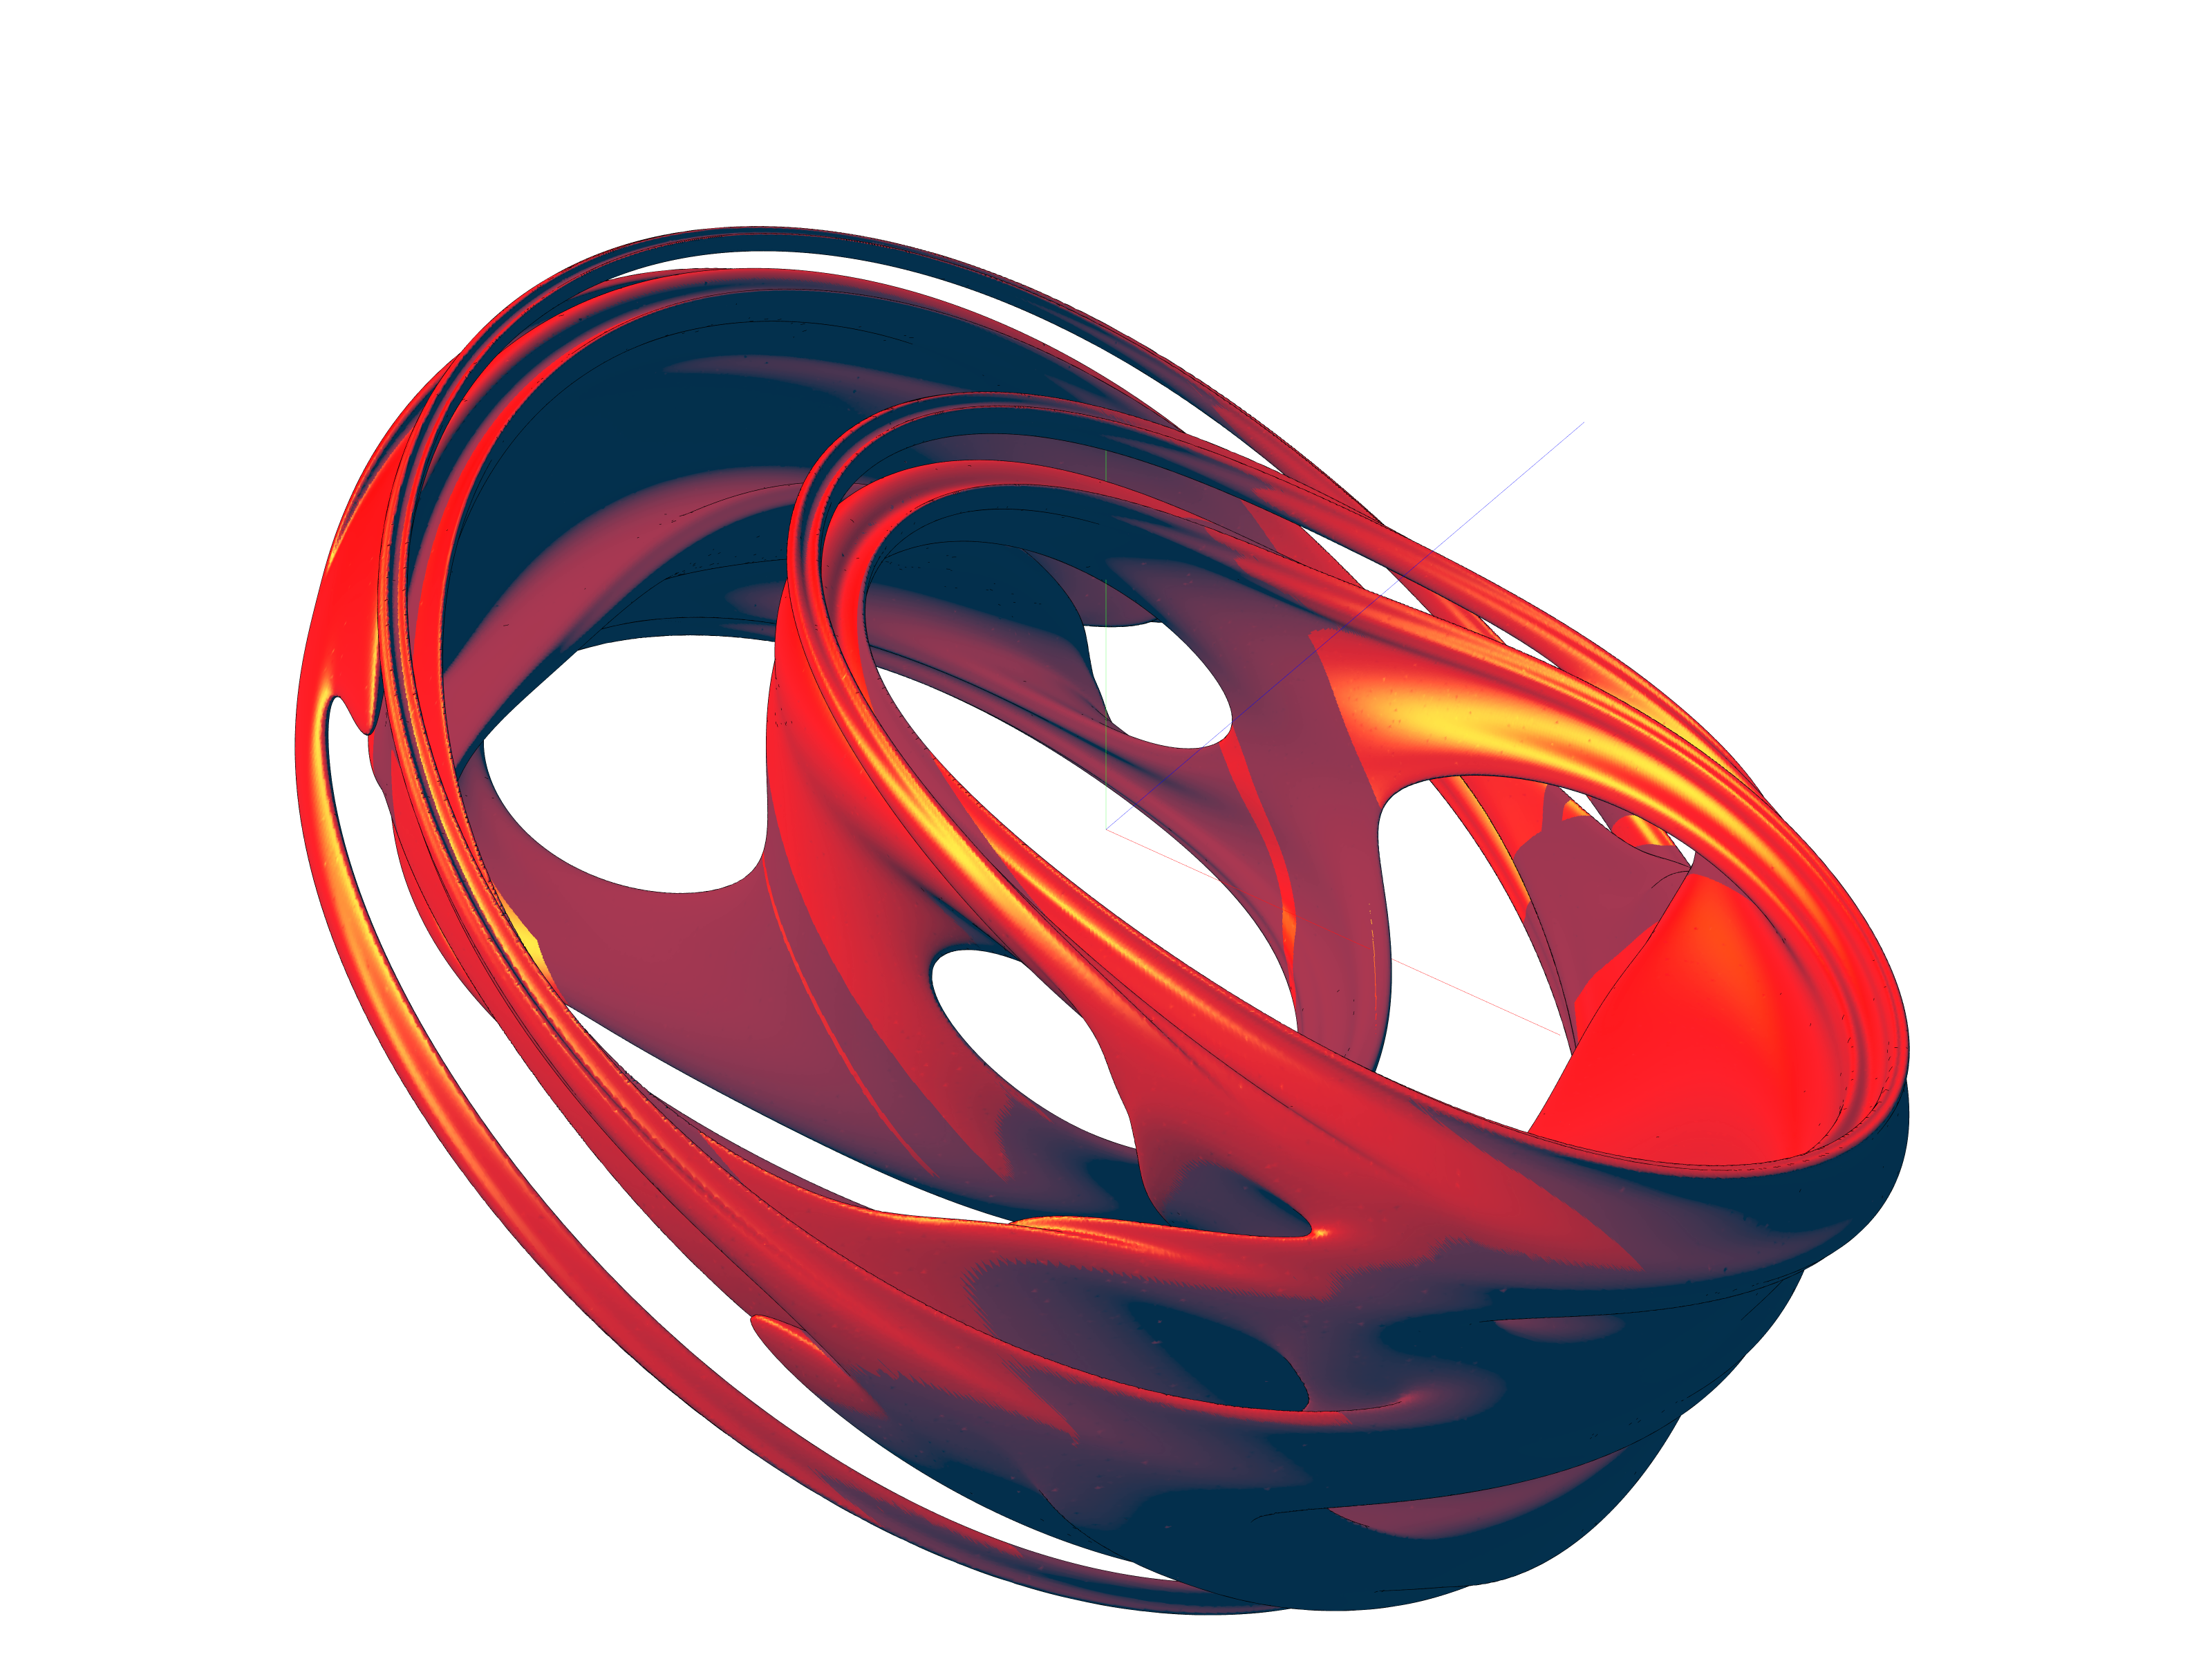
\includegraphics[width = 6 in]{quint_z2_c.png}
  \caption{A rendering of a $3$D slice of the $5$D Julia set.
The iterative equation is $A^{\prime} = A^2 + D$, where $D = (0.3, 0.5, 0.4, -0.2, 0.8)$.
The set is calculated using the new multiplication operator, although the traditional multiplication operator generates the same set as well.
}
\end{figure}

\begin{figure} 
\centering
  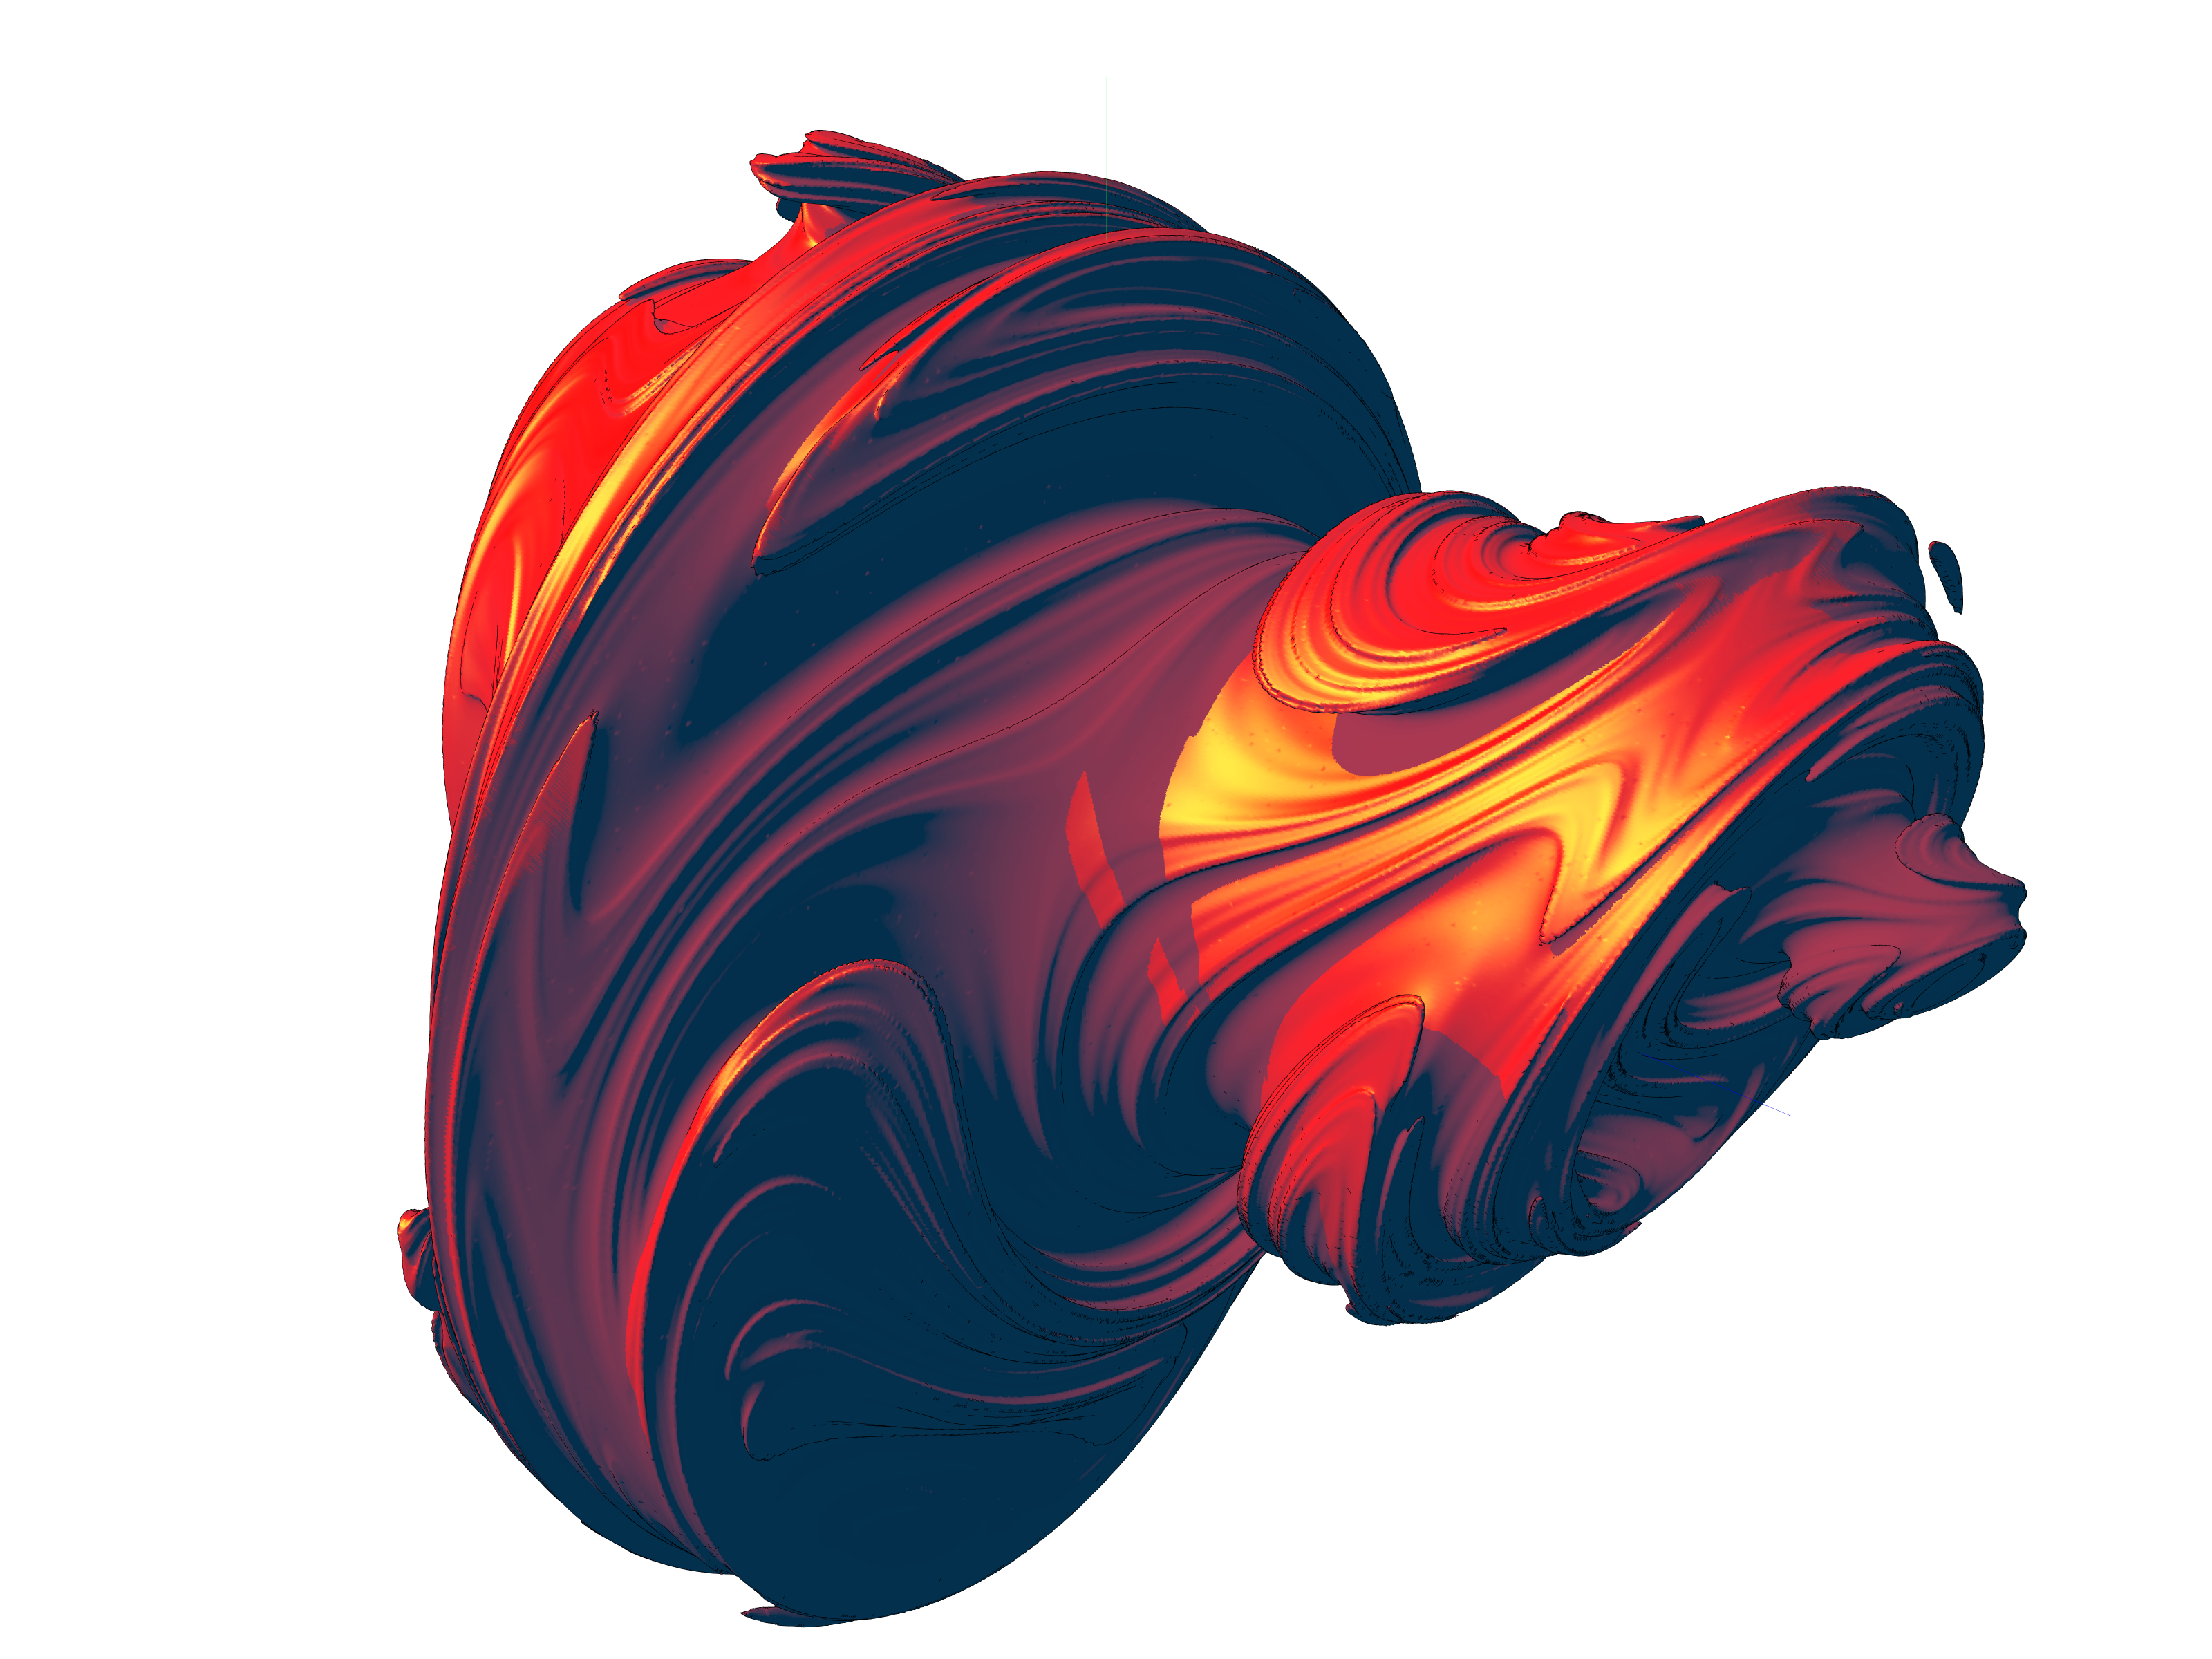
\includegraphics[width = 6 in]{quint_z3_c.png}
  \caption{A rendering of a $3$D slice of a $5$D fractal set.
The iterative equation is $A^{\prime} = A^3 + D$, where $D = (-0.3, -0.5, 0.4, -0.2, 0.1)$.
The set is calculated using the new multiplication operator, although the traditional multiplication operator generates the same set as well.
}
\end{figure}










\begin{figure} 
\centering
  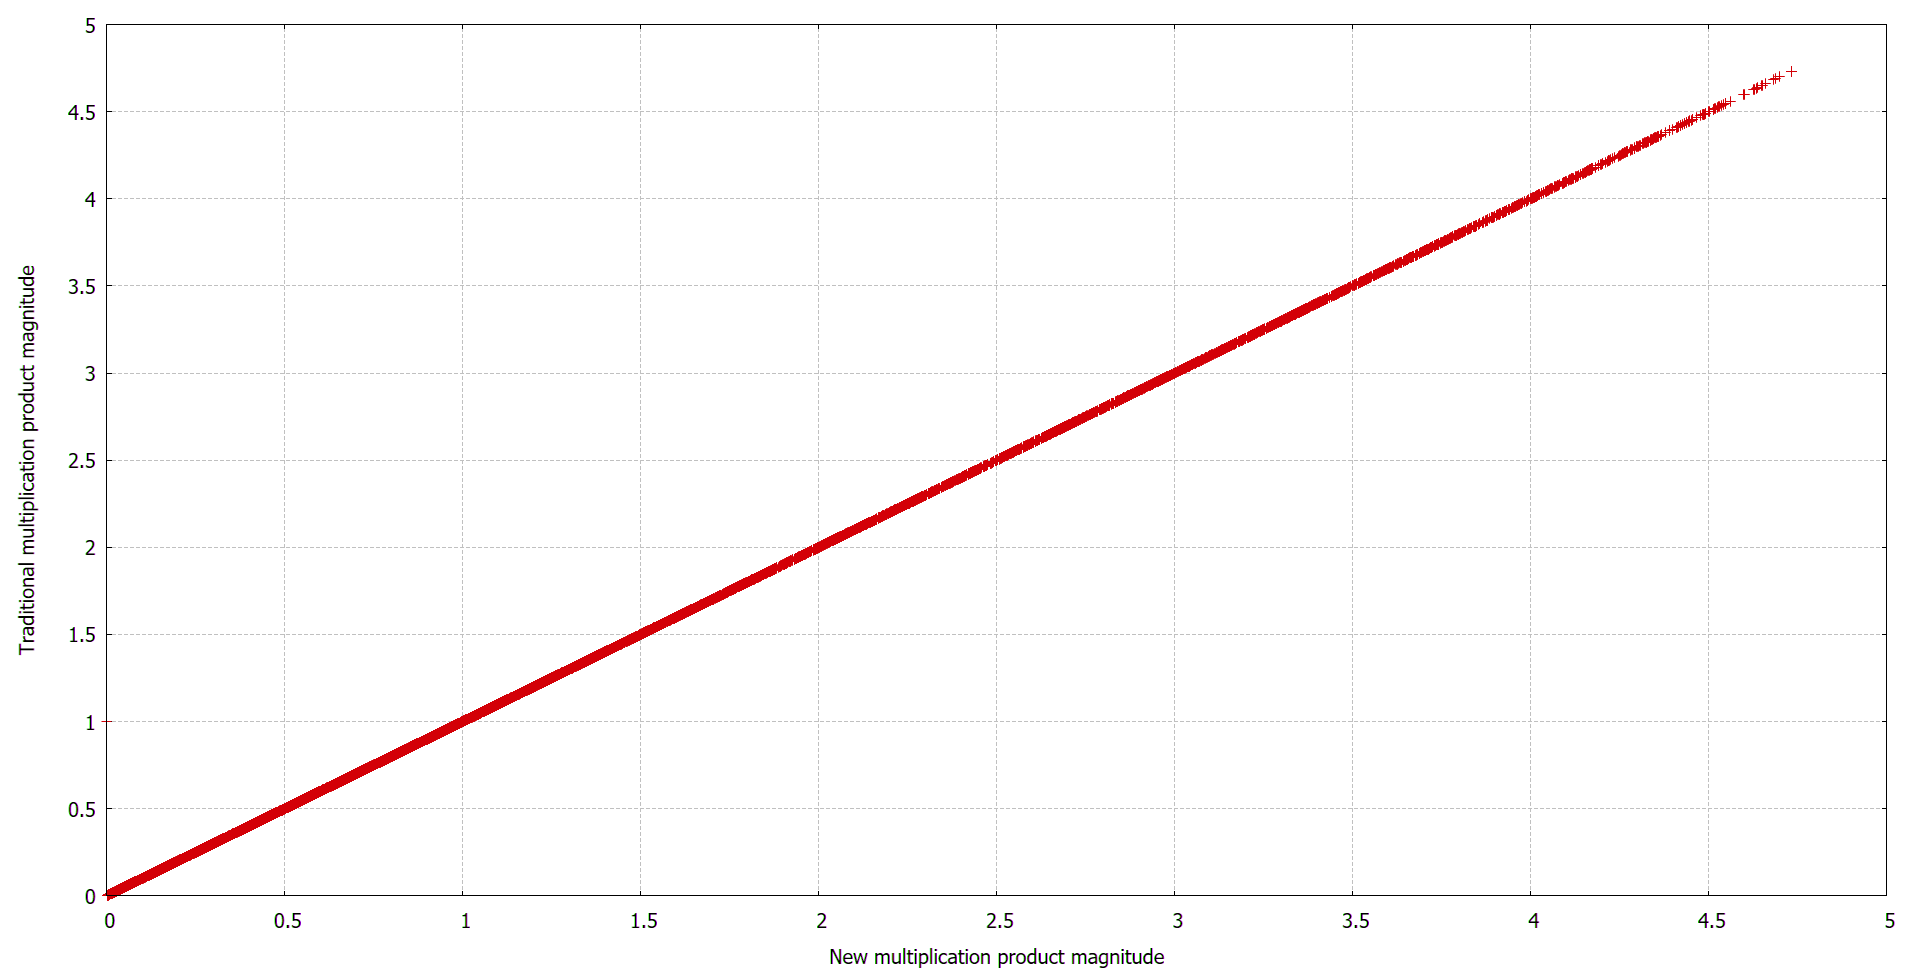
\includegraphics[width = 6 in]{a2_magnitude.png}
  \caption{A graph that compares the new multiplication product's magnitude to the traditional multiplication product's magnitude.
Note that the data form a straight line, which means that the products' magnitudes are equal.
The iterative equation is $A^{\prime} = A^2 + D$.
}
\end{figure}


\begin{figure} 
\centering
  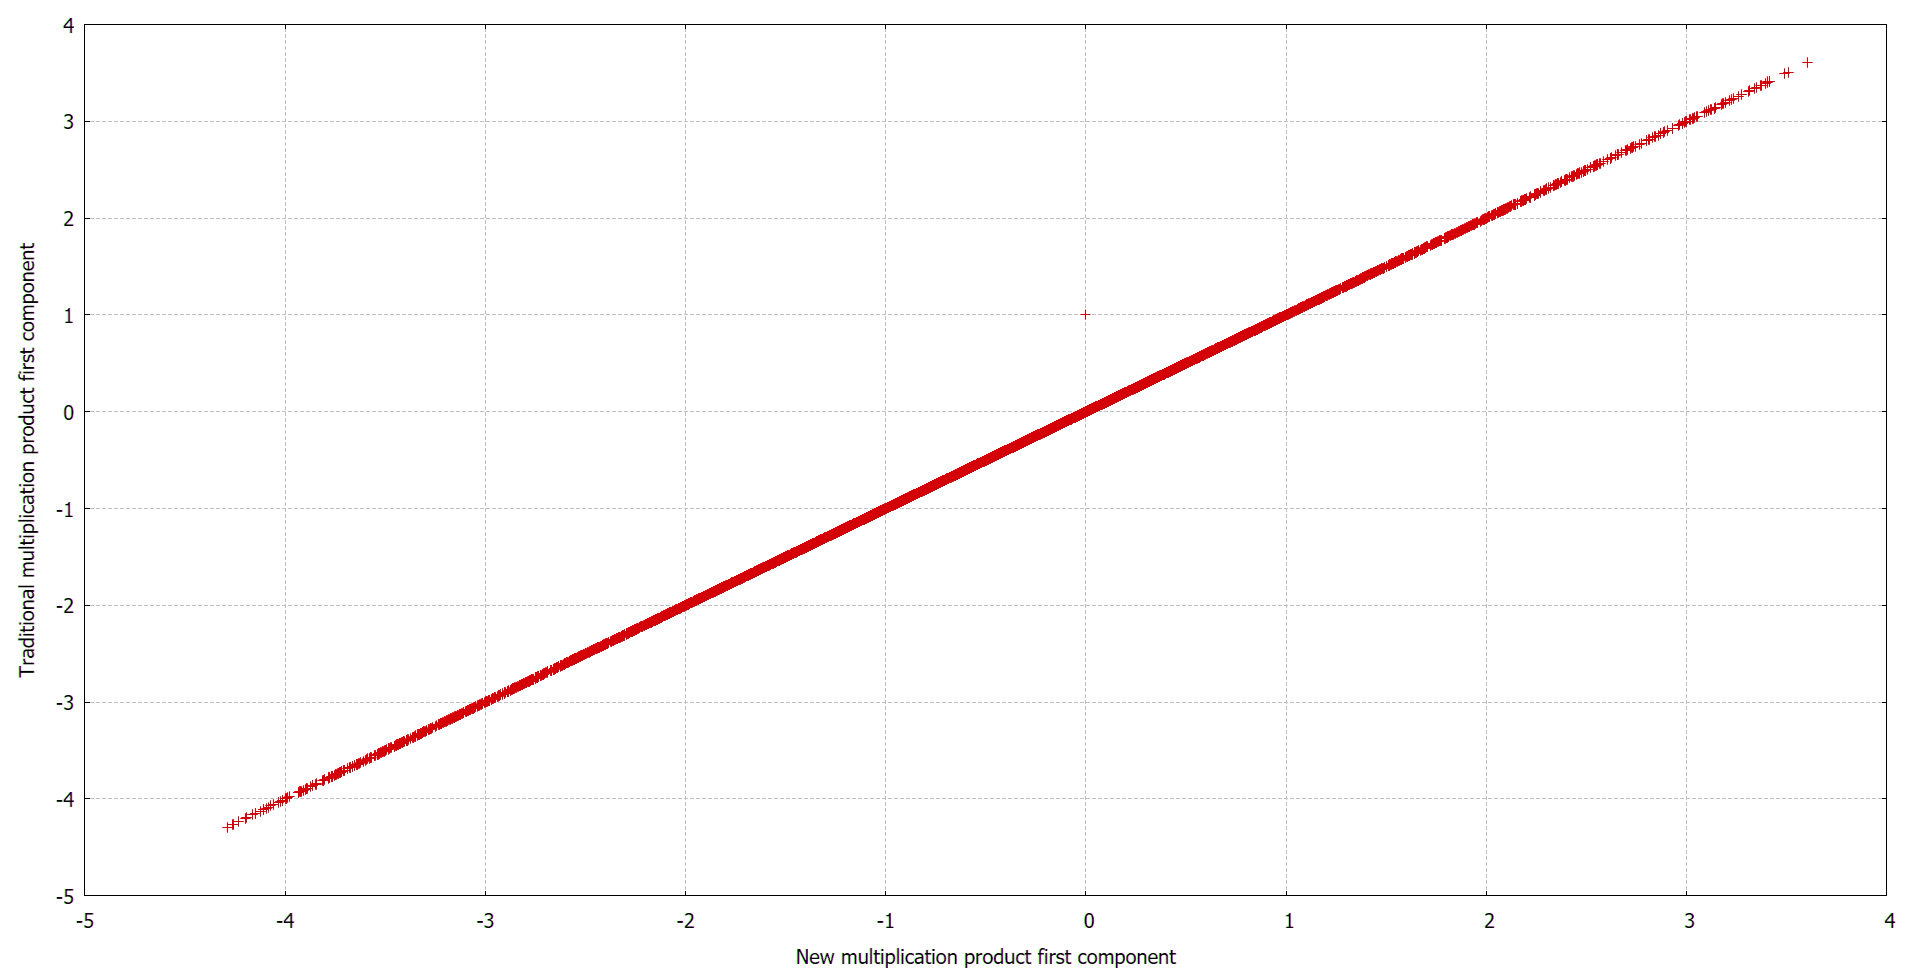
\includegraphics[width = 6 in]{a2_first_component.png}
  \caption{A graph that compares the new multiplication product's first component to the traditional multiplication product's first component.
Note that the data form a straight line, which means that the products' first components are equal.
The products' other four components are also equal.
The iterative equation is $A^{\prime} = A^2 + D$.
}
\end{figure}


\begin{figure} 
\centering
  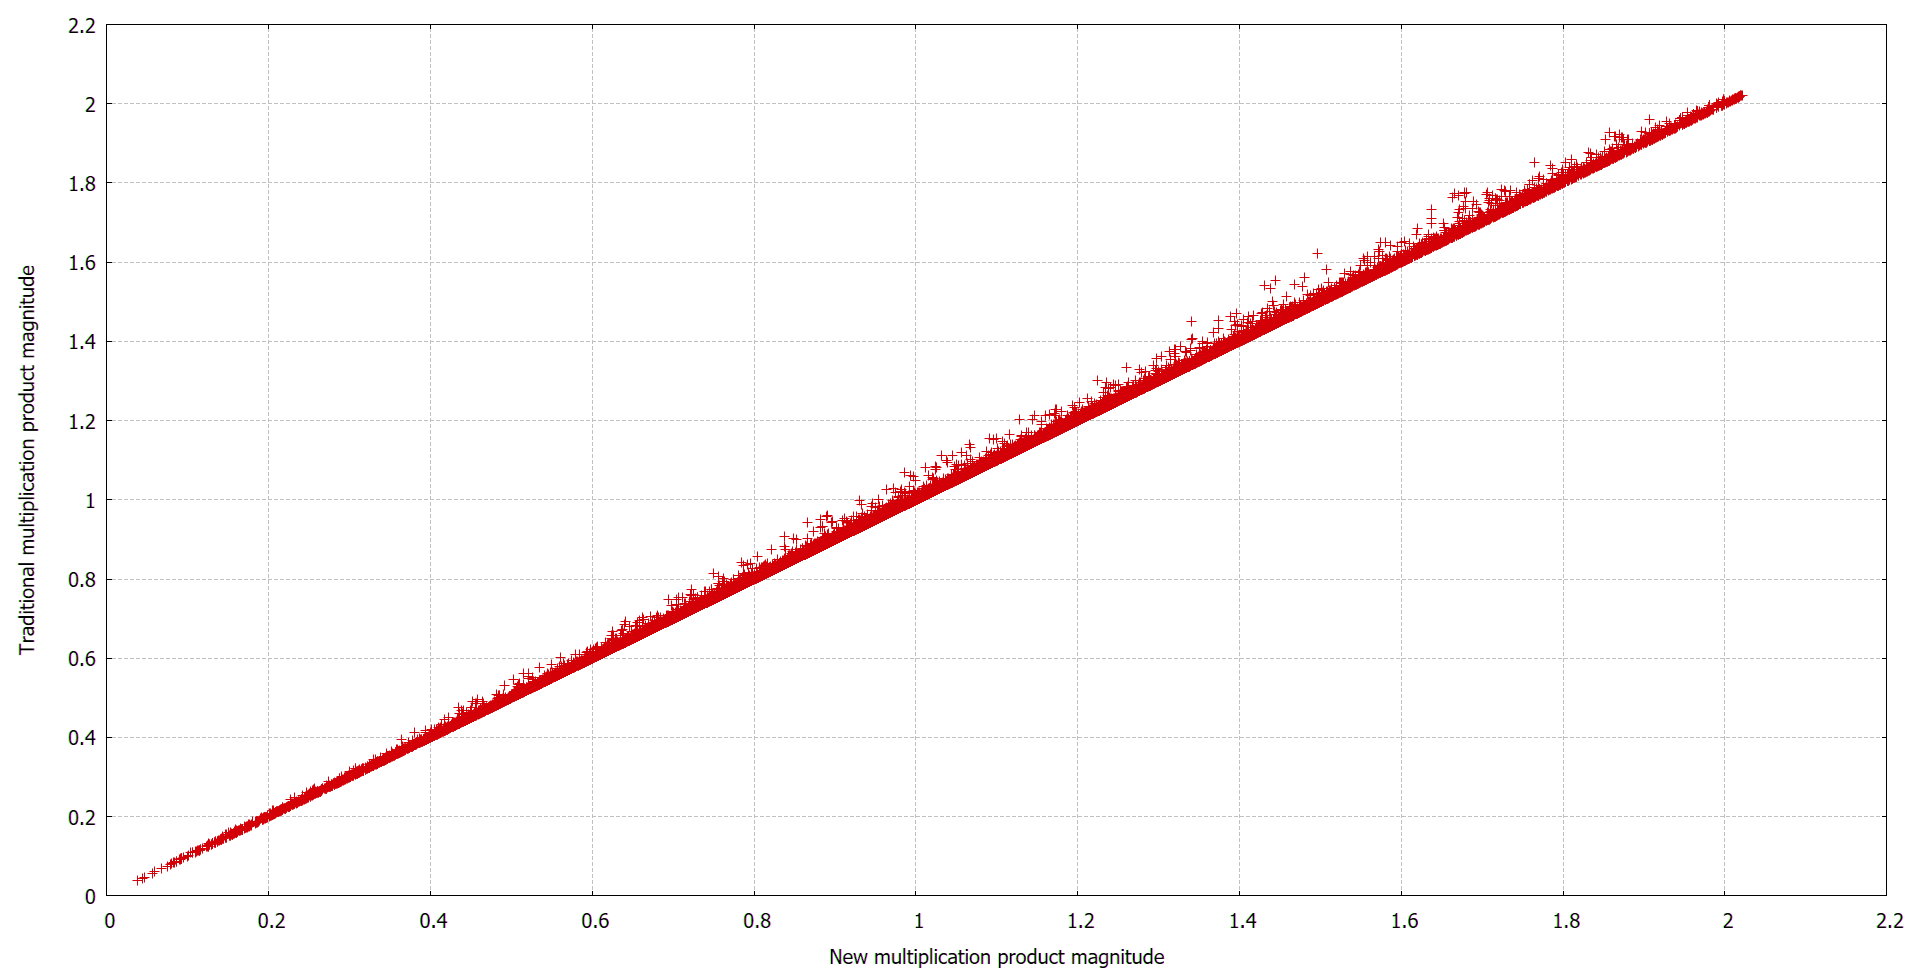
\includegraphics[width = 6 in]{sinz_c_magnitude.png}
  \caption{A graph that compares the new multiplication product's magnitude to the traditional multiplication product's magnitude.
Note that the data form a straight line, for the most part, which means that the products' magnitudes are equal.
The iterative equation is $A^{\prime} = \sin(A) + D \sin(A)$.
}
\end{figure}


\begin{figure} 
\centering
  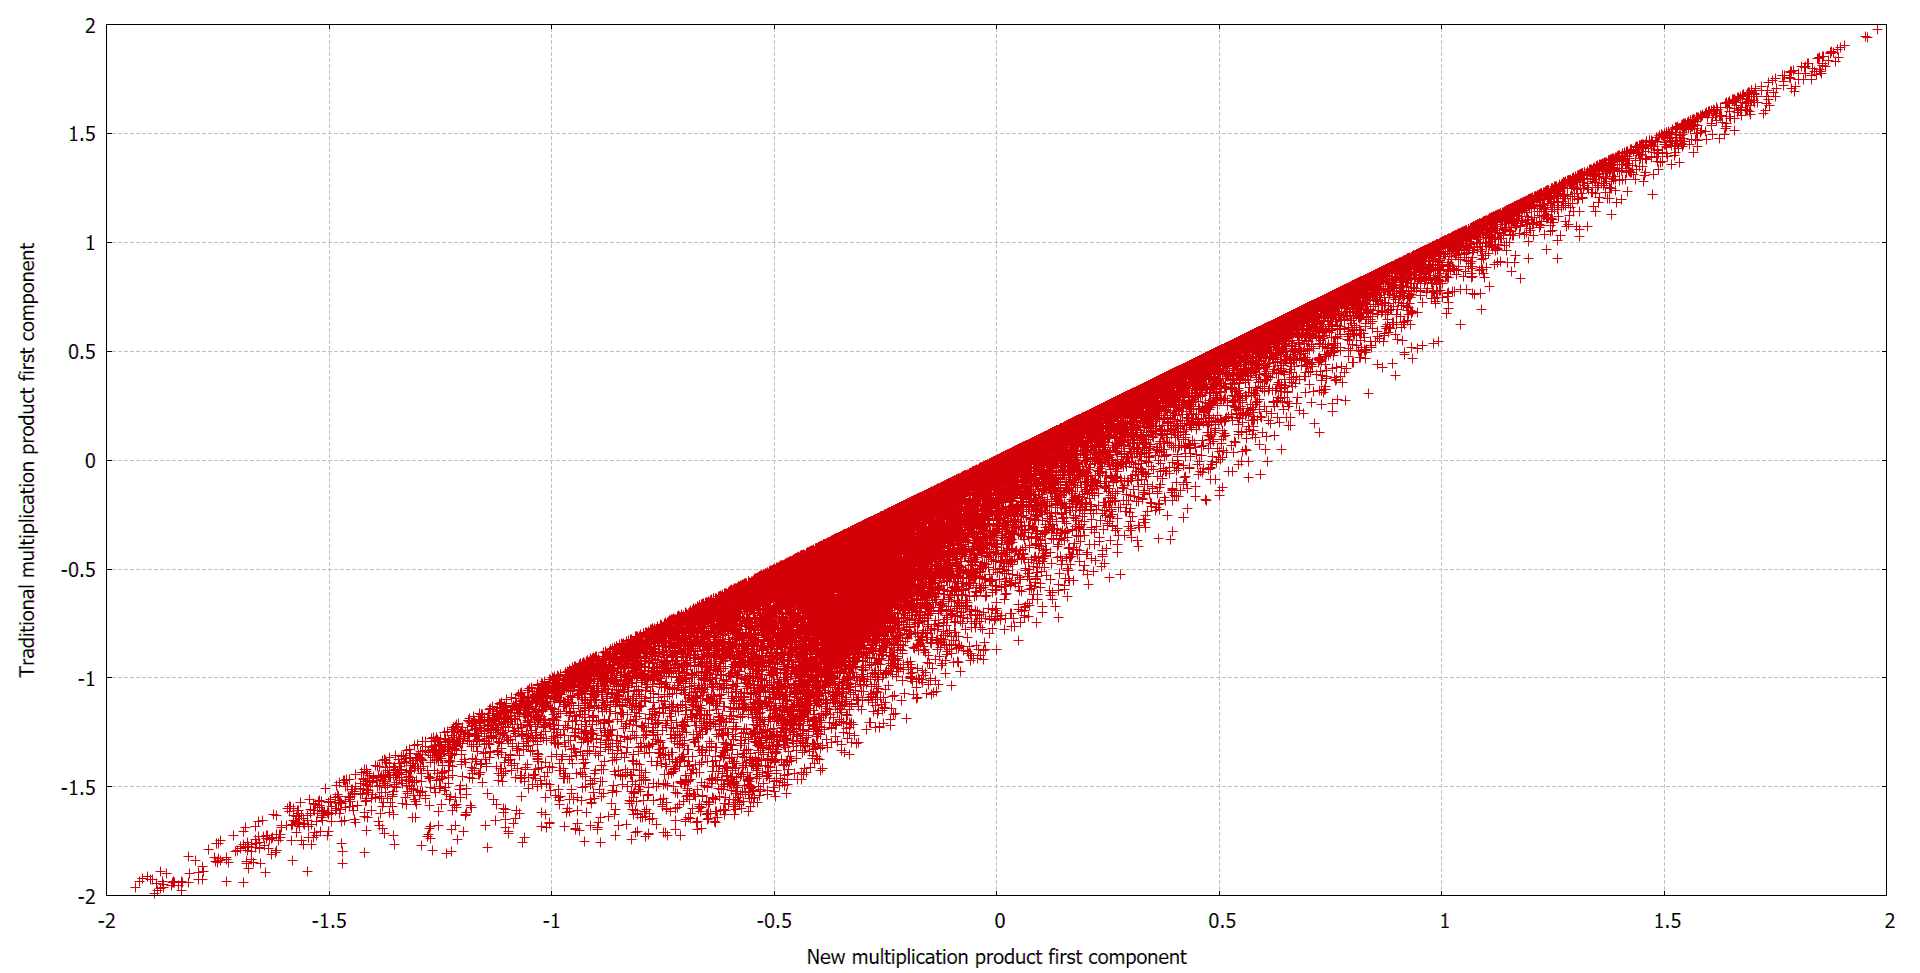
\includegraphics[width = 6 in]{sinz_c_first_component.png}
  \caption{A graph that compares the new multiplication product's first component to the traditional multiplication product's first component.
Note that the data do not form a straight line, which means that the products' first components are not necessarily equal.
The products' other four components are also not necessarily equal.
The iterative equation is $A^{\prime} = \sin(A) + D \sin(A)$.
}
\end{figure}





\begin{figure} 
\centering
  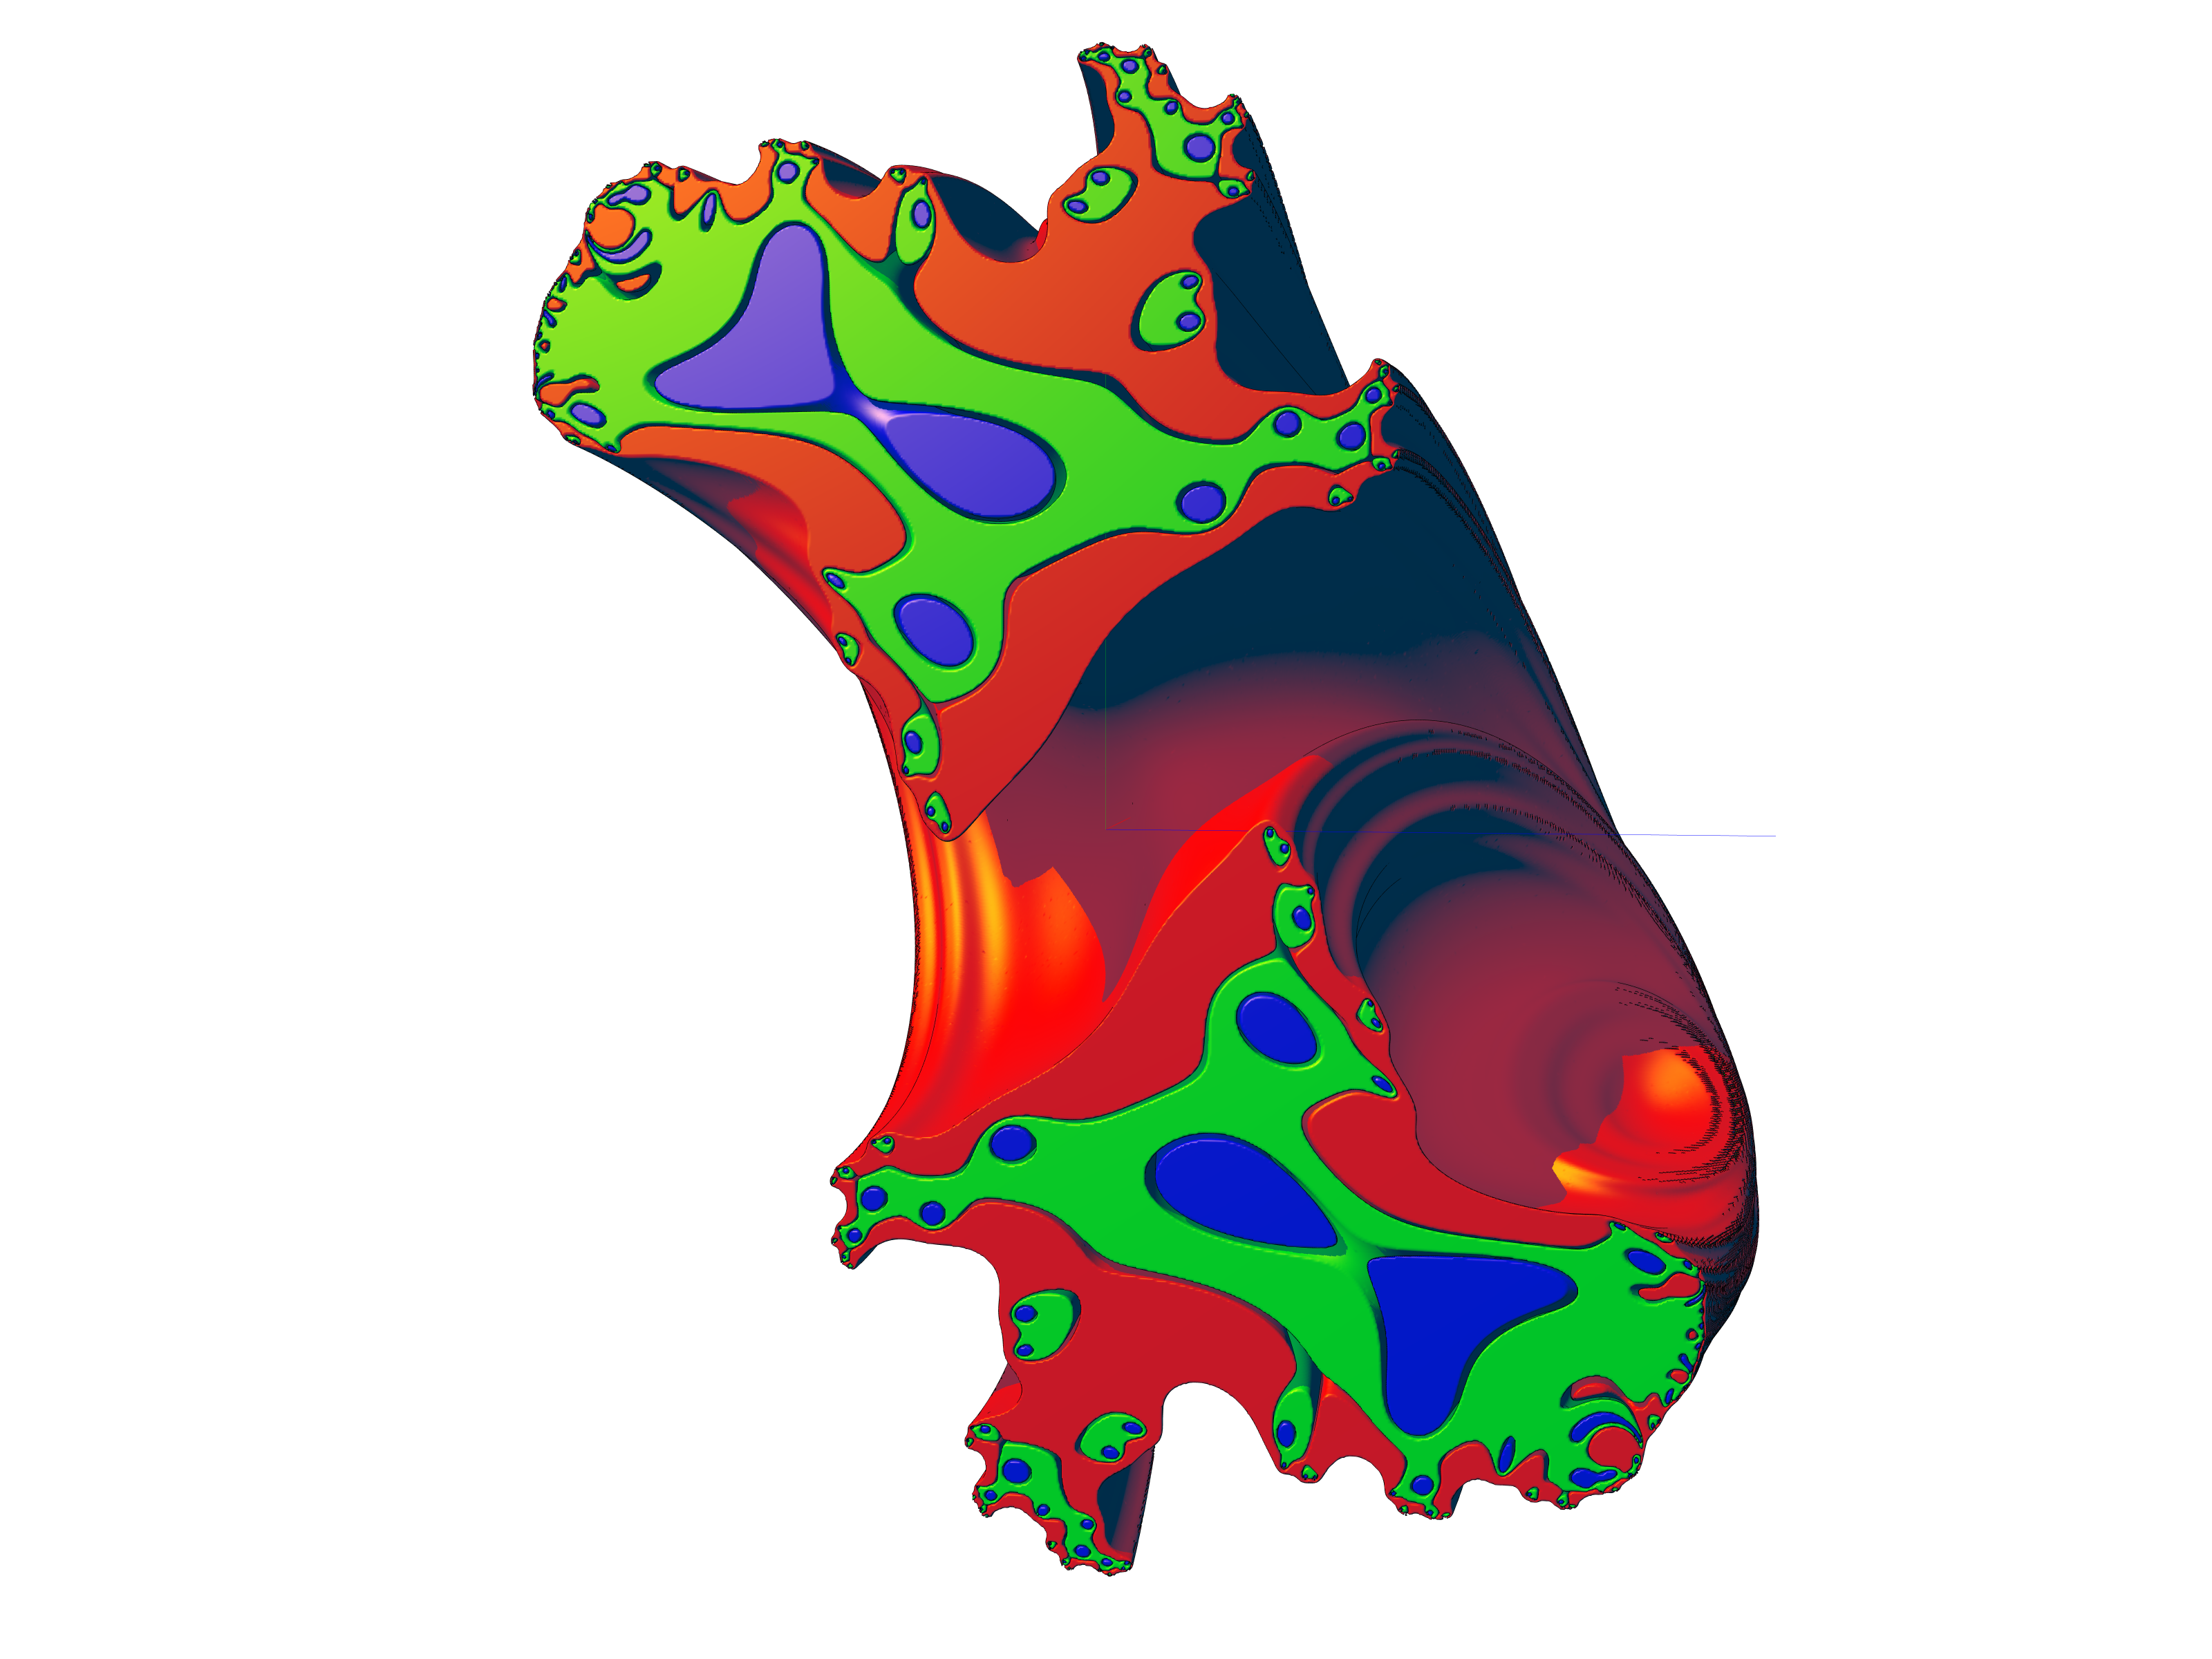
\includegraphics[width = 6 in]{rgb2.png}
  \caption{A rendering of a $3$D slice of the $5$D Julia set.
The iterative equation is $A^{\prime} = A^2 + D$, where $D = (0.3, 0.5, 0.4, 0.2, 0.1)$.
The $3$D slice is cut in half, and multiple isosurfaces are used to show internal detail.
The set is calculated using the pow() function, although both the traditional multiplication and new multiplication operators generate the same set as well.
}
\end{figure}






\begin{figure} 
\centering
  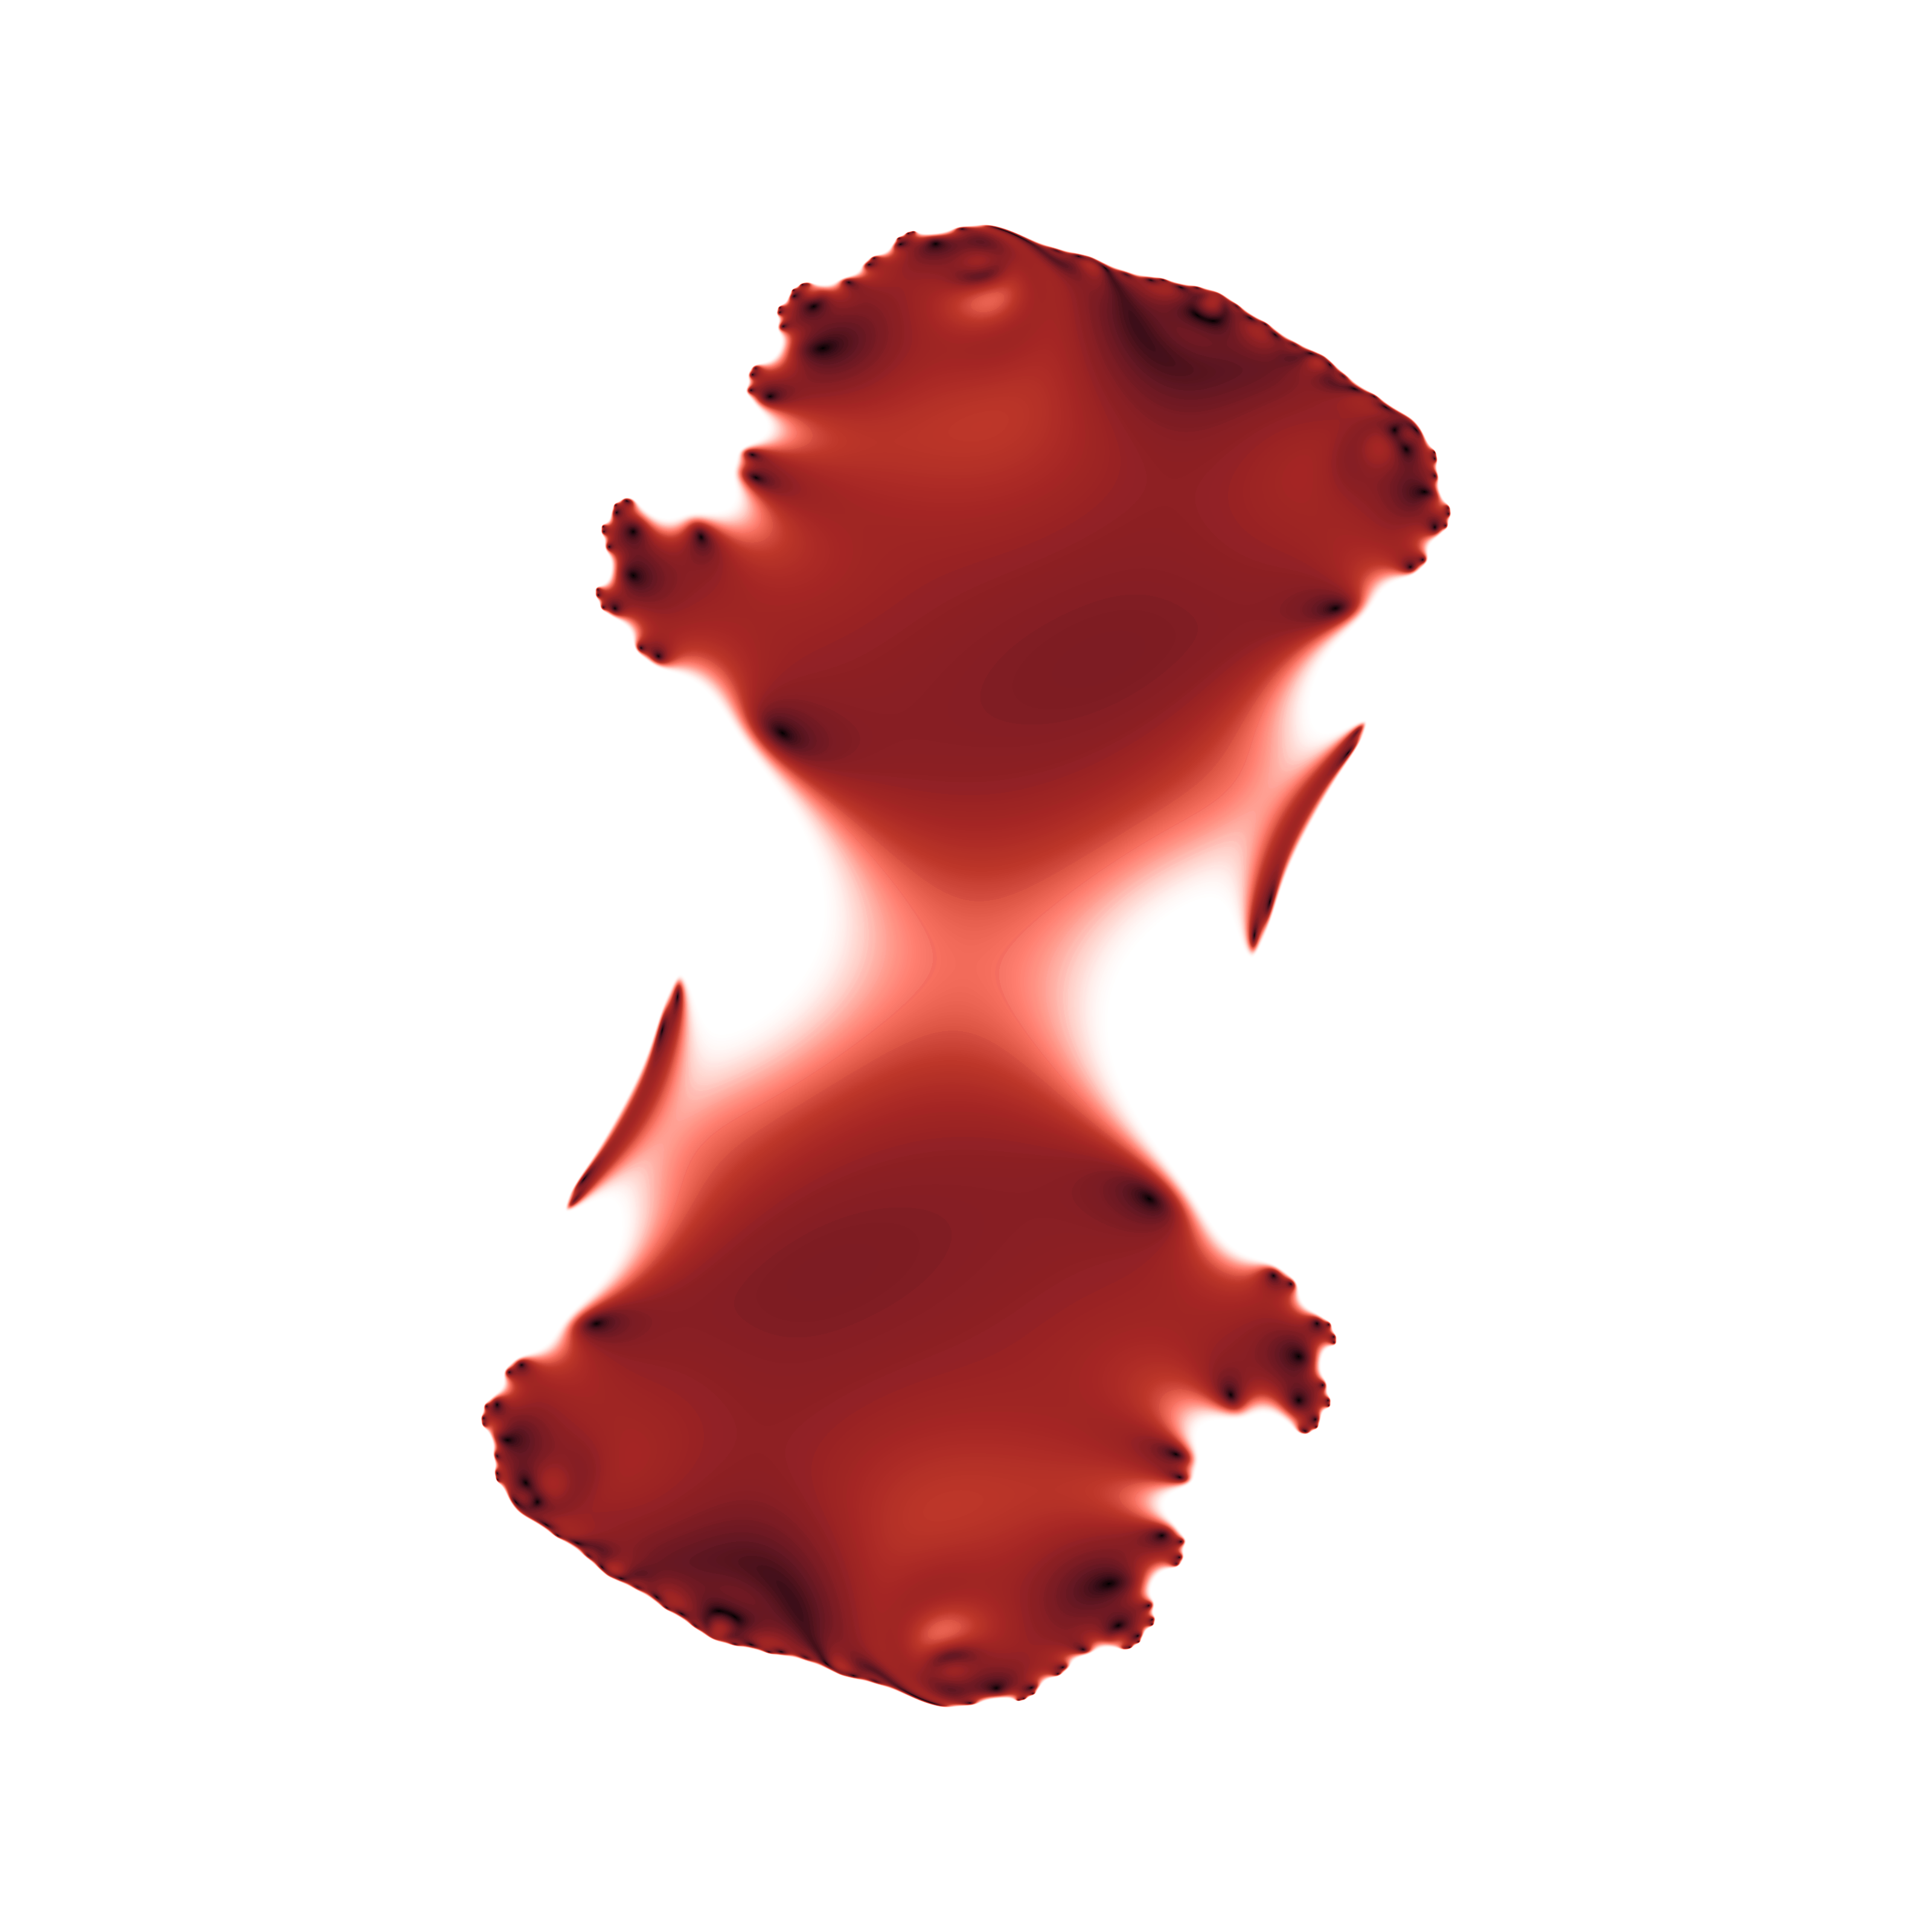
\includegraphics[width = 6 in]{16d_pow2.png}
  \caption{A rendering of a $2$D slice of a $16$D fractal set.
The iterative equation is $A^{\prime} = A^2 + D$, where $D = (0.2, 0.2, 0.3, 0.2, 0, 0.1, 0.1, 0, 0, 0.2, 0, 0.1, 0.3, 0, 0.2, 0.2)$.
The set is calculated using the pow() function, although both the traditional multiplication and new multiplication operators generate the same set as well.
Note that the intensity of each pixel is a reflection of the magnitude, with respect to the threshold value.
That is, pure white pixels lie outside of the set, and rest of the pixels lie within the set.
Pure black pixels correspond to zero magnitude.
}
\end{figure}


\begin{figure} 
\centering
  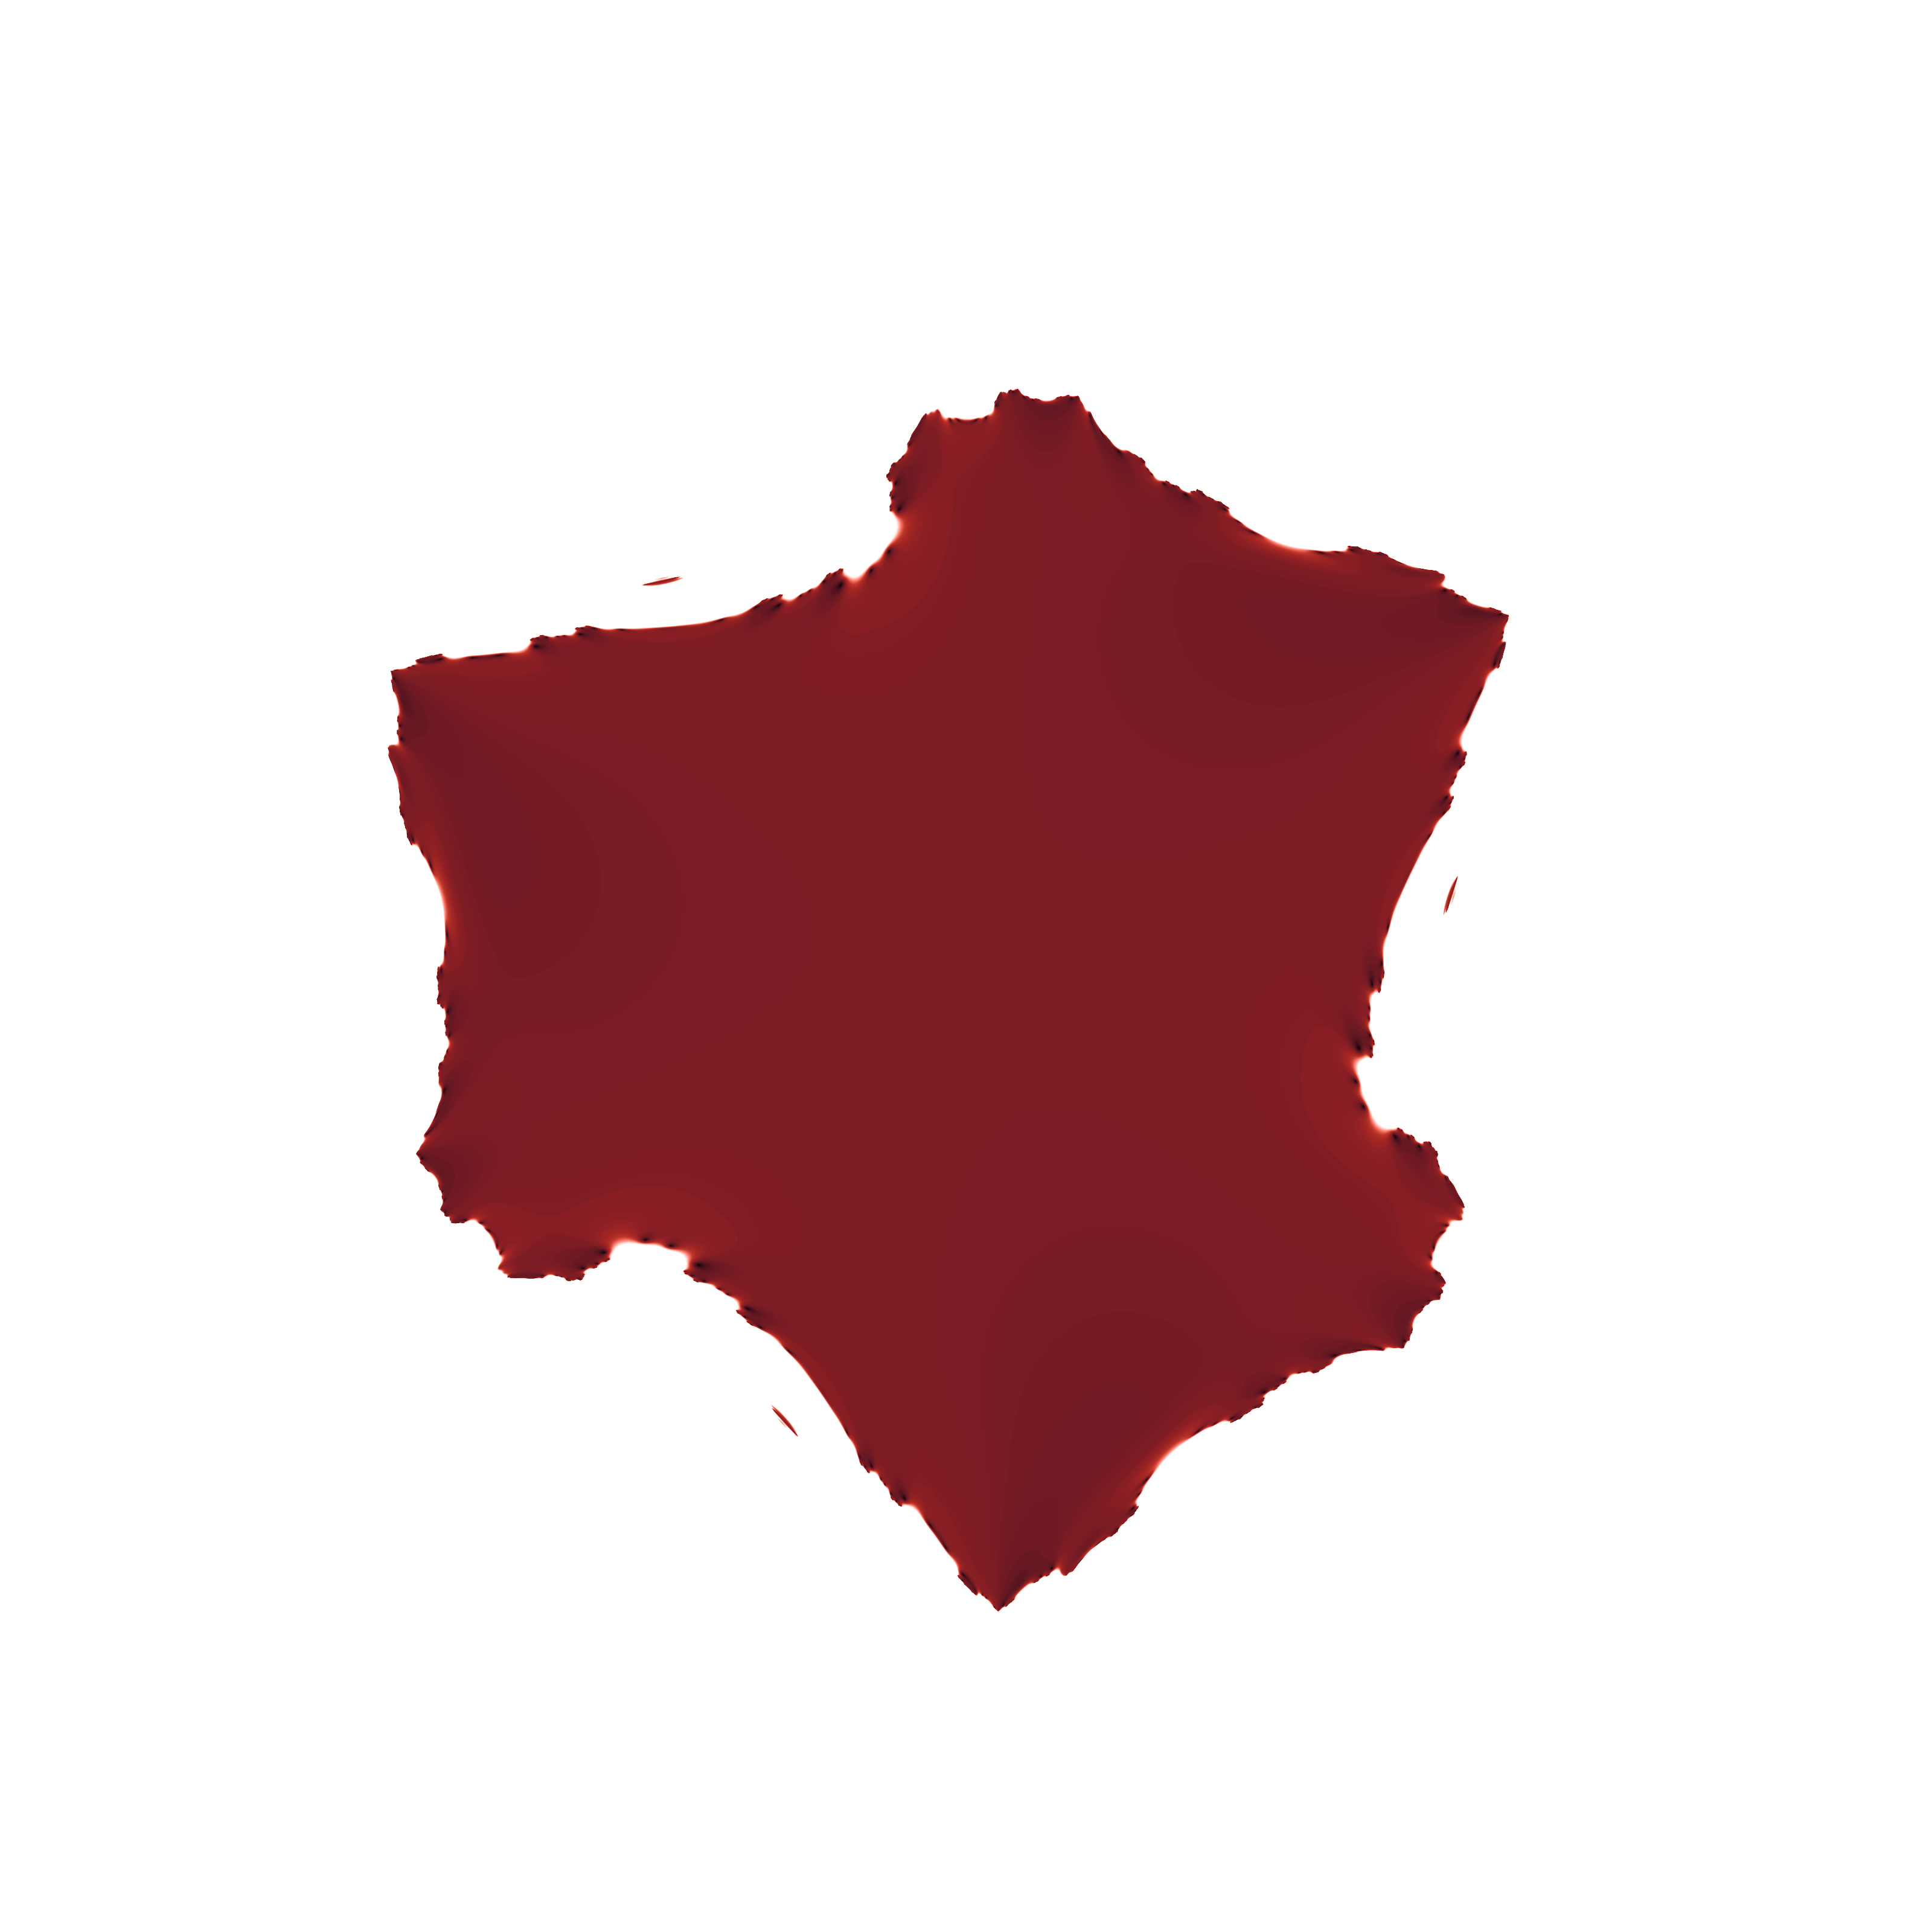
\includegraphics[width = 6 in]{16d_pow3.png}
  \caption{A rendering of a $2$D slice of a $16$D fractal set.
The iterative equation is $A^{\prime} = A^3 + D$, where $D = (0.2, 0.2, 0.3, 0.2, 0, 0.1, 0.1, 0, 0, 0.2, 0, 0.1, 0.3, 0, 0.2, 0.2)$.
The set is calculated using the pow() function, although both the traditional multiplication and new multiplication operators generate the same set as well.
}
\end{figure}




\begin{figure} 
\centering
  
\includegraphics[width = 6 in]{16d_pow5_5.png}
  \caption{A rendering of a $2$D slice of a $16$D fractal set.
The iterative equation is $A^{\prime} = A^{5.5} + D$, where $D = (0.2, 0.2, 0.3, 0.2, 0, 0.1, 0.1, 0, 0, 0.2, 0, 0.1, 0.3, 0, 0.2, 0.2)$.
The set is calculated using the pow() function.
Note that the exponent is not an integer.
}
\end{figure}



\begin{figure} 
\centering
  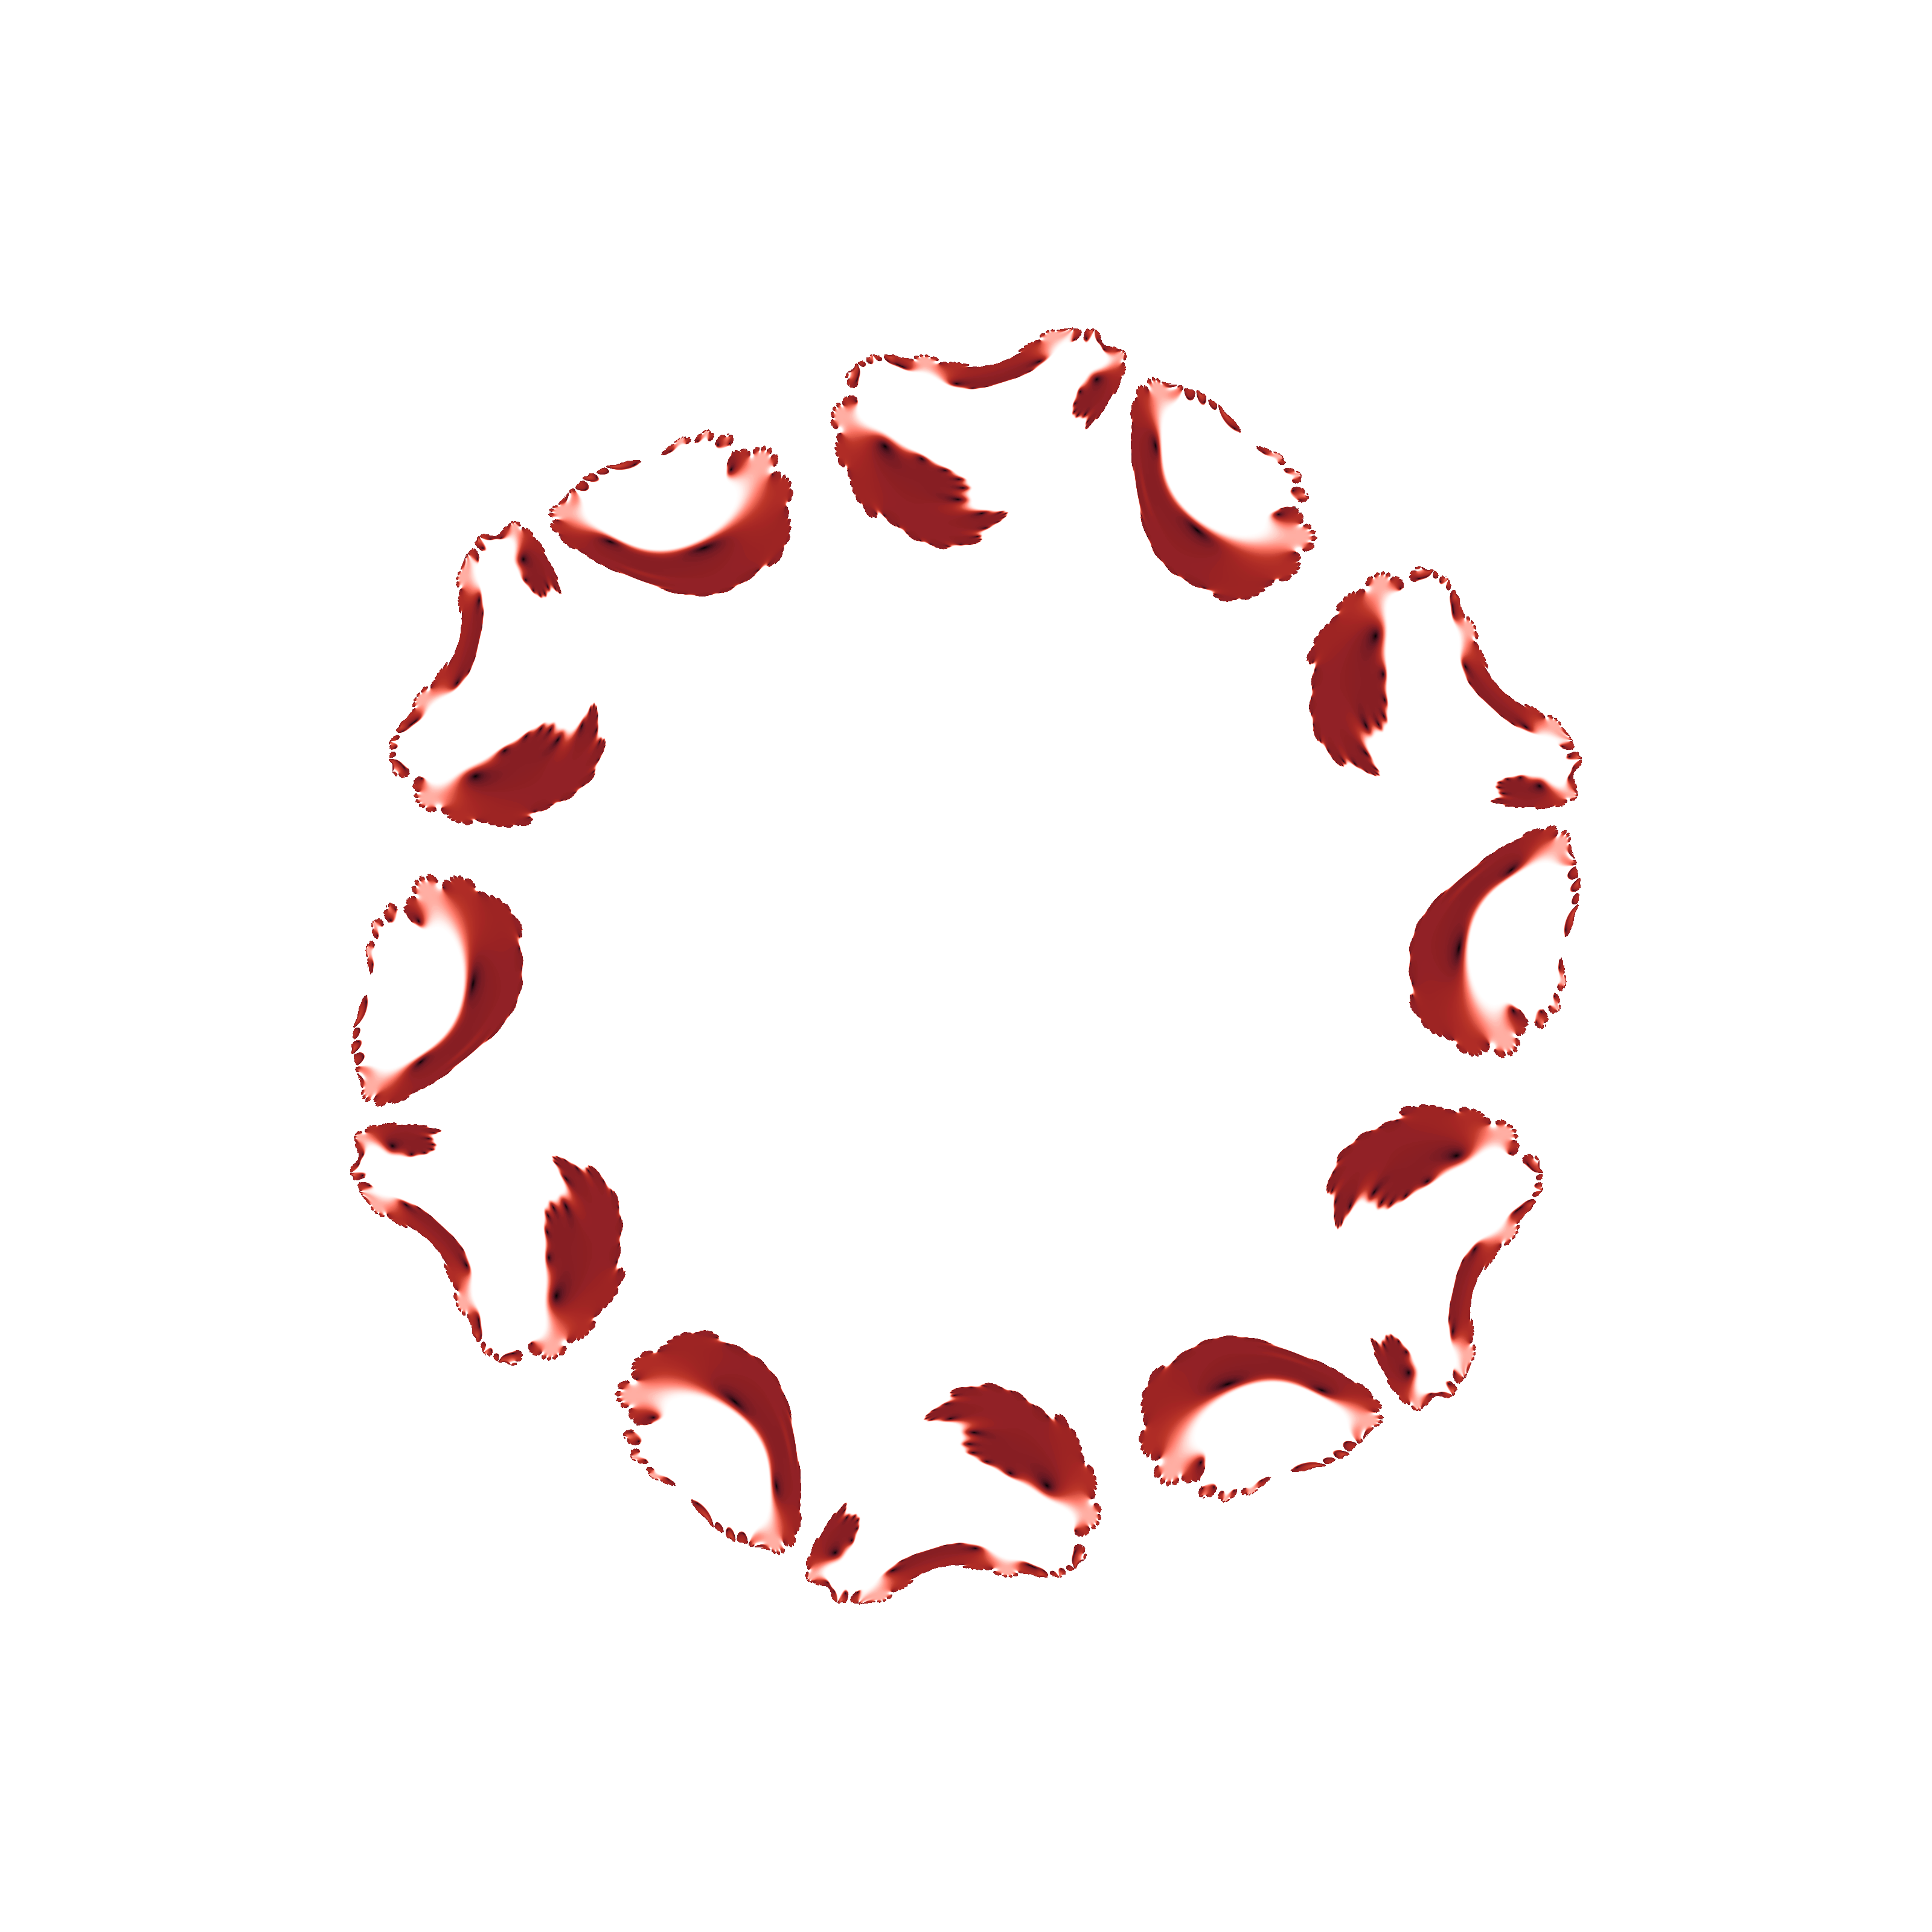
\includegraphics[width = 6 in]{16d_pow6.png}
  \caption{A rendering of a $2$D slice of a $16$D fractal set.
The iterative equation is $A^{\prime} = A^6 + D$, where $D = (0.2, 0.2, 0.3, 0.2, 0, 0.1, 0.1, 0, 0, 0.2, 0, 0.1, 0.3, 0, 0.2, 0.2)$.
The set is calculated using the pow() function, although both the traditional multiplication and new multiplication operators generate the same set as well.
}
\end{figure}



\begin{figure} 
\centering
  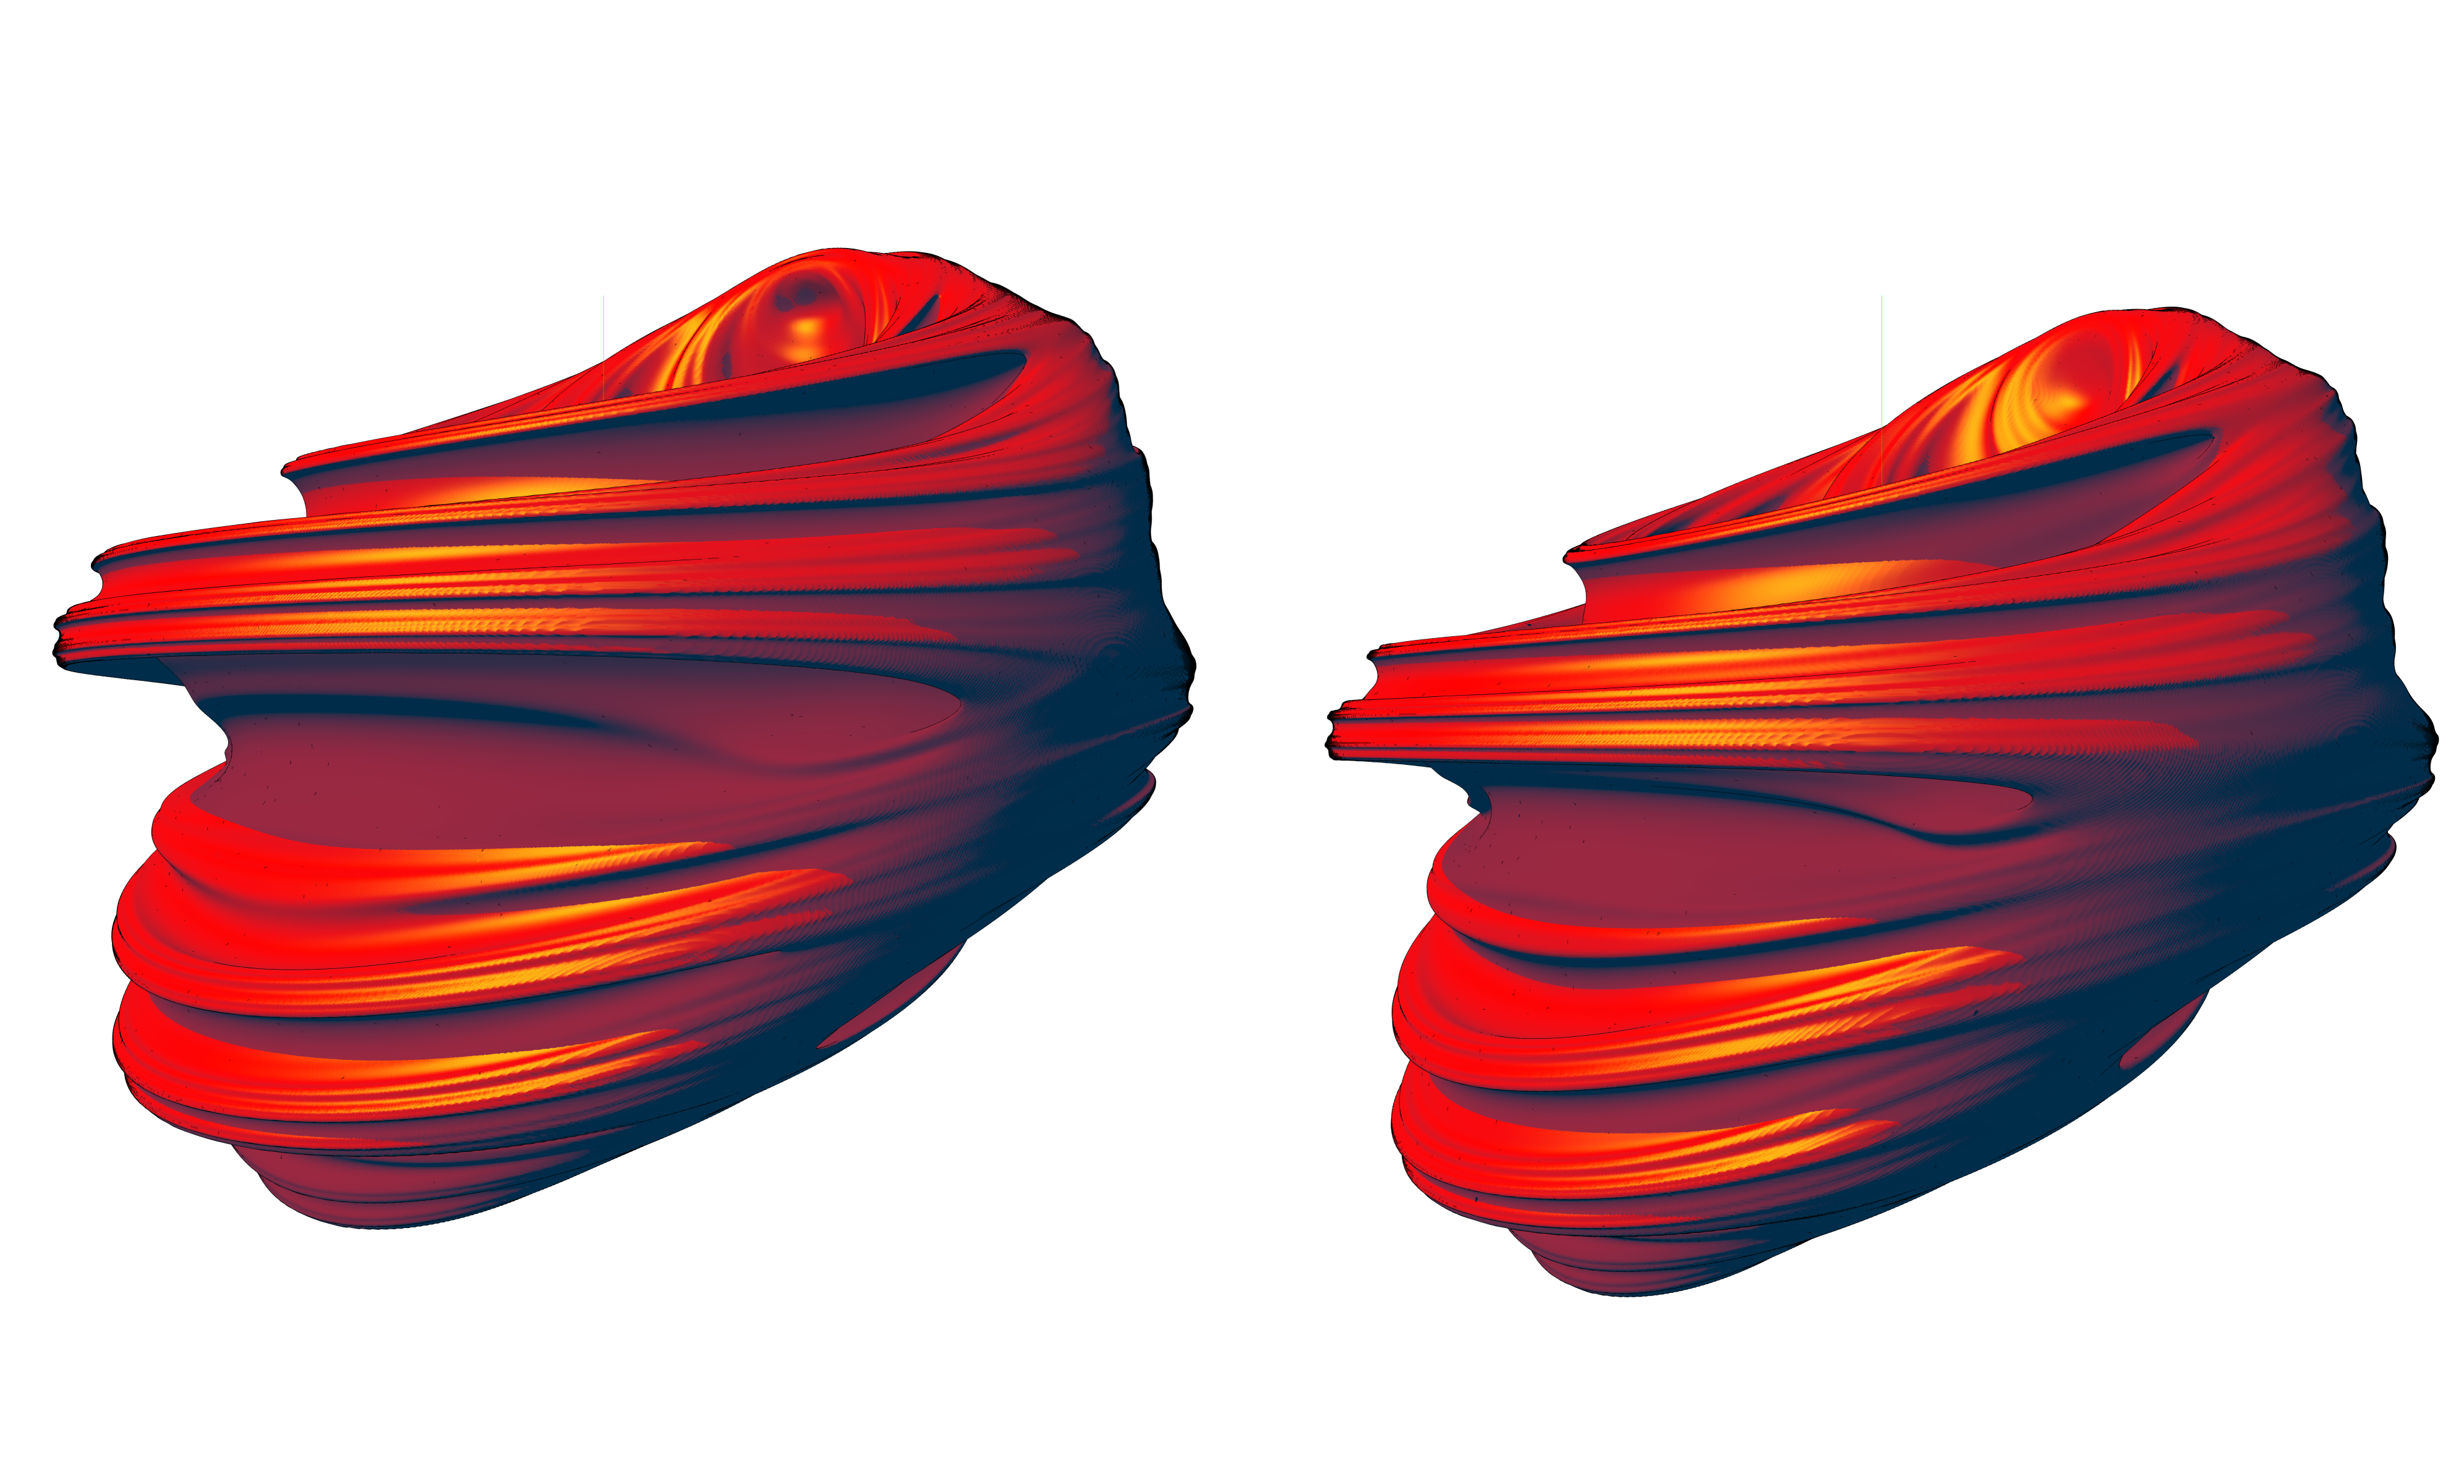
\includegraphics[width = 6 in]{ai_versus_ground_truth.png}
  \caption{A rendering of some $3$D slices of some $4$D fractal sets.
The iterative equation is $A^{\prime} = A^2 + D$, where $D = (0.3, 0.5, 0.4, 0.2)$.
The set on the left is calculated using artificial intelligence, and the set on the right is calculated using the traditional multiplication operator.
The aliasing in the meshes is due to the use of the standard linear vertex interpolation in the Scikit-image marching cubes implementation.
}
\end{figure}



\end{document}









